% This example An LaTeX document showing how to use the l3proj class to
% write your report. Use pdflatex and bibtex to process the file, creating 
% a PDF file as output (there is no need to use dvips when using pdflatex).

% Modified 

\documentclass{l3proj}
\usepackage{wrapfig}
\usepackage{subfig}
\usepackage{float}
\usepackage{listings}
\usepackage{pdfpages}

\usepackage{url}
\usepackage{appendix}
\begin{document}
\title{A Website Translation Service}
\author{Alasdair Campbell \\
	Andrei Mustata \\
	Paul Moore \\
        Stephen Hayton \\
	Wei Zhang}
\date{\today}


\maketitle
\begin{abstract}

Since the writing of the earliest manuscripts and documents there has been a
need for translation so that the people of the world could understand what had
been written or said, in their own native language. Translation is just as
relevant today as it was thousands of years ago, although the processes have
modernised considerably. The focus of this project is to create an online
presence and document delivery system for a freelance Glasgow-based natural
language translator. Our goal is to improve upon the translation websites
currently available and to give a unique, modern and fresh feel to translation.

\end{abstract}
\educationalconsent
\tableofcontents
\newpage
%==============================================================================
\begin{flushleft}
A foreword from our client, Jo\"{e}lle Cimatche.
\end{flushleft}	

\textit{``When I first met Dr Karen Renaud a few years back, little did I know I
would need a website of my own as a translation marketing tool since I have been
a member of a number of professional websites for translators and interpreters.
But over the years those marketing avenues have proved insufficient which caused
me to think it may be time to have a website of myself.\\
\\
So last year I got back in touch with Dr Renaud and we discussed the prospect of
my professional website. She arranged a meeting with a team of the students who
would be entrusted with the project of designing the website.
During that meeting, I was supposed to suggest my expectations to the team but
in reality, I had no idea how the website should look like. All I needed was a
website as a marketing tool. Computer science has always been a mystery to me,
so talking about a website was a daunting experience I was not prepared to
face.\\
\\
But shortly after the meeting had started, the team took turns in coming up with
attractive ideas concerning how they believed a good website should look like. I
was speechless. Those ideas were based on the languages I work in, methods of
payment, and how professional my dealings with current and future clients should
be.\\
\\
From the beginning of the project to the end, the team has been very patient as
I had to juggle between my work and family lives among others, and could not
always meet the deadlines when it came to provide them with the necessary
information pertaining to the website.
They have shown a high level of skills, team work and kindness that resulted in
what to me is an advanced type of professional website.
While my heartfelt thanks go to the team as a whole I want to express my
gratitude particularly to Alasdair who offered to temporary host the website
while in the making and Stephen (the spokesperson for the team) for his
promptness in answering my emails and putting up with my ignorance of Computer
science.\\
\\
Thank you again for this cutting edge gift that you served me on a golden plate.
I am for ever indebted to you guys and am already bragging over it to my
friends. I wish you all the very best in your studies and future career.''}
\begin{flushright}
-Jo\"{e}lle Cimatche, Translator at BethelTranslations.com
\end{flushright}
\newpage
%==============================================================================
\chapter{Introduction}
\label{chap:intro}
\textit{\small{This article assumes a basic general computing knowledge from the
reader. If any words or phrases are not understood, consult the glossary of
terms (Section~\ref{chap:gloss}) at the end of the document. All content is
owned by the authors of this document or is otherwise referenced in bibliography
(Section~\ref{chap:bibl})}}\\
\section{Background}
As part of our degree in third year we are tasked with a team project. This
relates to computing disciplines new to us and draws on knowledge gained from
the preceding two years at University. Teams were randomly assembled at the
beginning of the first semester and our team received this project, to create a website
providing a document translation service for a real client. It was a pleasing
allocation mainly due to the latter part of the task: the fact we would be
working with a real client. \\
\\
There are many translation services available on the Internet already, a simple
Google search for online translation returns around one hundred and fifty-nine
million results. We have looked into various different forms of translation and
interpretation websites during our research and have found pros and cons from
each. This vast number of existing websites creates a desire to compete 
with what's already available, by striving to improve on the other site's
shortfalls. We believe one of the key factors that makes a
modern website successful is a minimalistic design: one that offers simple and effective
functionality and is aesthetically pleasing. The combination of these factors 
means users are more likely to use the website after stumbling across it in a
search and this will, ultimately, give our client a larger customer base. To
clarify, we are not trying to re-invent the wheel with our project. We have used
frameworks and other open-source components in the development of our website.
The system is mainly built around the LAMP structure, i.e., Linux + Apache +
MySQL + PHP. We believed that these choices would lower the costs of an eventual
upgrade of the system, as opposed to having used some more exotic technologies
that come at the cost of losing the robustness and stability that we needed. We
aimed to maintain a user friendly look and feel at all times, and believe that
this is something we accomplished well. One of the facts that encourages this notion is the fact we
have created a simple 3-stage process in which users can register, upload
documents, and request languages to translate to.\\ 
\section{Aims}
Our aim was to develop a cutting edge software system to facilitate a functional document translation service for a
free-lance translator. It should allow customers to upload documents, request
one of the available languages to translate to, and submit a request for
translation. The translator should then be able to review those submitted
documents and send a quote to the customer for the job to be translated. If
happy, the customer should then be able to pay for the job(s) via PayPal, and
then receive their translated document after a specified period of time.
Additional required features of the website will be discussed later. 


\section{Motivation}
This bespoke web-based service builds on our
client's existing business model, with the specific aims to bring about an
expansion in her company, while also facilitating an improvement to her working
practice as a whole.

Listed below are a few important points on why using a software system to manage
documents and to keep track of discussions and tasks has advantages over the
current manual system, and why our client has been motivated to seek a software 
solution:

\begin{itemize}
	\item
	It makes {\bf planning} deadlines easier, since computers are better than humans
	at taking large amounts of data and comparing, adding, etc.;
	\item
	It makes {\bf file management} easier;
	\item
	It increases {\bf productivity} - due to the two above points, the
translator now employs an organised system and has more time to devote to the
translations\end{itemize}

By having all the job details clearly stated and planned, the customers are
encouraged to pay more attention and to take it more seriously. It also
introduces the notion of accountability on both sides - customer and translator.
Having a detailed log of all the documents delivered to customers makes keeping
track of all the activities easier to do. By using an electronic payment system,
the risk of having unpaid jobs is eliminated. It also gives the business a more
professional look and leaves our client less vulnerable to hacking attacks as
opposed to other methods of payment. One of the principal requirements of our
website is support PayPal for payment of services. \\

Bethel Translations is a worthwhile use of our time for many reasons. We are helping
to produce a system that will be used by a local businesswoman with a young family.
This provides a great sense of achievement for our team as something we are building is
helping others in their daily life. The experience we have working with a real external
client will be invaluable come graduation and when we are seeking employment. Having
already been through an entire software engineering process will be a great asset to us.
This project gives us a chance to learn new skills with web frameworks and website
development languages such as PHP, HTML and CSS, which again is advantageous in
the jobs market and for future projects.
Additionally, there is motivation to succeed and to be better than the competition.
As discussed there are hundreds of thousands of other translation services - this means
that for our service to succeed there must be an advantage to using our system over
another. This has motivated us into nding the best possible solution for our client and
the website.

\section{The Translator}
An essential part of our requirements gathering process was the first meeting
with our client, the translator, Jo\"{e}lle Cimatche. Our team had been forewarned by our
supervisor that the translator was not very ``technically minded'', so we
endeavoured prepare questions that did not assume a particular aptitude for
computers. It's fair to say that after reading the initial brief for the project
we made assumptions as to the needs of the translator, addressing the problem
from our viewpoint. Realising we should expect to review these assumptions
during the process of working on the requirements capture is a valuable lesson
for future employment. Working with an individual or organisation, firmly on the
periphery of Internet technology adds it's own challenges, particularly during
the requirements capturing process. During the meeting, we discovered our client
had a very basic understanding of word processing applications and the Internet. 
This presented us with an additional challenge. We couldn't
simply relay technical jargon to the translator and expect her to provide useful
feedback. Not only that, our team would have to create a very easy-to-use administrative
interface to the website that she could pick-up easily.\\
\\
As we advanced the development of the website, we were careful to be very clear
and straightforward when updating the client on our progress. We accomplished this
mainly through emails containing concise, clear and jargon free status updates
on the website progress. These updates had been sent at important stages of
development such as the transition from the design inception to the early
implementation. The essence of our approach was to produce a website which delivered the requirements of our client. When we felt there
was a need to query the client on certain aspects of the
web-site's implementation, we emailed her without hesitation and she was quite often happy to
accommodate these changes. It seemed that she was prepared to grant us some
degree of trust with creating her website, which certainly helped, but we still
sought her opinion of most changes that took place. Arguably then, communication
with our client has been crucial to the design of this website. Our
communication was put to the test when we needed the client to sign up for her own
web server. We had to prepare a lengthy, detailed and broken down walk through
of how to purchase website hosting. For an average user of the Internet, this
task would have been far less demanding. However, our client's expertise in this
domain required far more patience. \textbf{Figure 1.1} helps to illustrate the
challenge we had. Known as Roger's Bell Curve, it describes an ``adoption rate curve'' for a percentage of
users of new technologies. Relating this to our situation, our client would be at the far right end of the spectrum, in the 16\% of
users described as "Laggards" in the graph.\\
	
\begin{figure}
\begin{center}
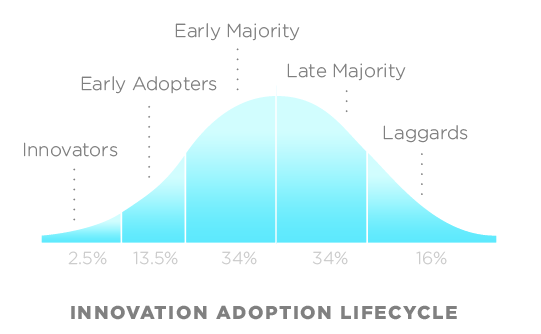
\includegraphics[scale=0.6]{DiffusionOfInnovation}
\caption{Roger's bell curve, source: http://en.wikipedia.org/wiki/File:DiffusionOfInnovation.png}
\end{center}
\end{figure}

Another point to consider is how users actually come to accept and use a
new technology, and the factors that influence such a decision. \textbf{Figure
1.2}, otherwise known as the Technology Adoption Model (TAM) provides a
graphical realisation of this.
\footnote{\url{http://en.wikipedia.org/wiki/Technology\_acceptance\_model}} The model
suggests that when users are presented with a new technology, a number of
factors influence their decision about how and when they will use it, notably:

\begin{itemize}
\item Perceived usefulness (PU) - This was defined by Fred Davis as "the degree
to which a person believes that using a particular system would enhance his or
her job performance".
\item Perceived ease-of-use (PEOU) - Davis defined this as "the degree to which
a person believes that using a particular system would be free from effort"
(Davis 1989).	
\end{itemize}

From our early meetings with our client, we believe we can make well informed
assumptions about these two aspects. Since the client has especially contacted
the University to ask for such a website to be implemented, and the fact she
currently has no online presence already, it is our understanding that she
believes this website or new system will definitely enhance her job performance.
We have some reservations about her perceived ease of use however. As is
explained earlier, she is very inexperienced with Internet technologies in
general and may not feel entirely comfortable when faced with the new system for
the first time. It is our main task to achieve simplistic, user friendly design
that she can learn to use as quickly as possible and overcome any early doubts
about the system. We believe that the website brings benefits to her work-flow,
that far outweigh our initial challenge of working with a novice user, although it is
certainly a trade off we have to be mindful of. 

\begin{figure}
\begin{center}
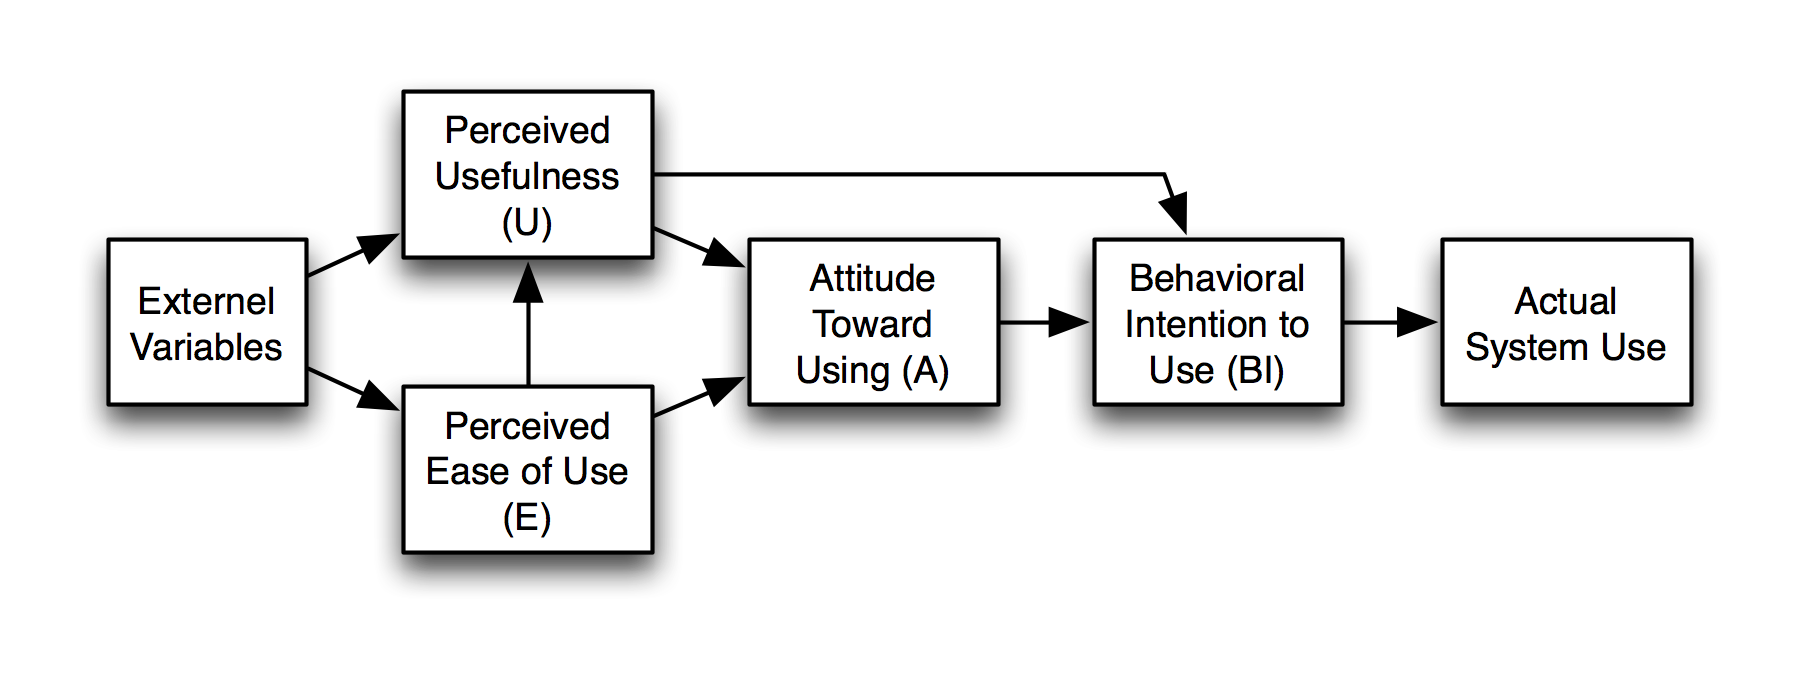
\includegraphics{tam}
\caption{Technology Adoption Model, source: \small{http://en.wikipedia.org/wiki/File:Technology\_Acceptance\_Model.png}}
\end{center}
\end{figure}

Reflecting on our experiences in our project, working with the client has not
been exceptionally easy. One of our main challenges is that our client is a
novice computer user. Quite ironically, it has been a task for us to translate
regular computing jargon into layman's terms in order for them to understand.
This was critical in our requirement gathering process. In spite of this
additional challenge, which teams working on other projects might not face, at
no point did we feel this was discouraging. When we eventually graduate and face real world software projects, it won't
always be technically minded people like ourselves we deal with, it will people
who are more similar to our client. It will provide us something to draw upon
when we are asked to recount our experiences in future interviews. The
opportunity to work with a real client could serve us as great preparation for
working life.\\
\\
Our project lives on the Internet. Ten years ago, the Internet was everywhere,
but now it's even more so. It's a rapidly evolving area where new technologies
and new techniques are developed very quickly. These have been made easy to use
by anyone, regardless of: computer knowledge, nature of their device (mobile or
desktop) or their operating system. All they need is an up-to-date web browser -
arguably an easy requirement to fulfil, since most of them update
automatically. From this we can surmise there is a large audience within the
reach of our project. This is a considerable motivating factor for everyone in
the team.\\

\section{Preliminaries}
To understand this report it is necessary to understand that we do not have to
implement a translation algorithm. We are providing customers with an interface
to send documents to be translated by a professional translator for a fee, and
then returned in the chosen translated language using the same web interface. To
understand the process that we have devised it would be advantageous to have a
simple understanding of how a database works. As mentioned earlier, we have
adopted several frameworks in our project development. These include Bootstrap
(CSS, HTML), CodeIgniter and PHPMyAdmin (all of which are discussed in
Section~\ref{chap:design} later). These frameworks provide advanced
functionality which will, in most instances, not be necessary for our project
and will not be utilised. Conversely, it allows us to demonstrate that we are
professional software developers and that we are capable of software re-use.

\section{Outline}
The remainder of this report will go into more detail on the background research
of our project, expand on our motivation and set out our group organisation and
project plan. After this we will detail our design ideas and methodologies,
before moving on to document our implementation, testing and evaluation. We will
then discuss any problems encountered and the results of our evaluation before
revealing the final status of the project, giving a detailed outline of the
deployed site including any graphics and information relating to Bethel
Translations.
 

%==============================================================================
\chapter{Design}
\label{chap:design}
\section{Requirements Gathering}

At the beginning of our project we met with the client and our supervisor to
discuss the project requirements. Our client currently works for
an agency, on a largely ad-hoc basis, and is looking to create her own translation
business. To this extent she wishes to have a website built to allow her to gain
an online presence in translation and to digitise the process of receiving and
sending documents. We were armed with a long list of questions and ideas for
the meeting and a transcript is included as an appendix.\\
\\
As software developers naturally would when creating anything from scratch, our
team looked for similar websites already in existence. We identified common
useful features of each, those features that were not so useful, and
listed some we thought could be useful but simply did not exist in any of the
sites we examined. One recurring theme we noticed in a majority of similar
translation websites was that the home page was very cluttered and full of text.
Due to this, the process that the user had to follow to obtain some
translation of a document was not very clear. Instead, they were met with
various registration options, other services and annoying advertisements.
\textbf{Figure 2.1} is a prime example of such bad design practices. It is
cluttered, unclear and unattractive to potential customers. The most intriguing
thing about the website in particular is that is ranked \textit{first} in a
Google search for the term "document translation". Rather alarmingly it seems
this site has prioritised search engine optimisation over actual usability, or
they have spent most of their budget paying to be rated first. Whilst being
rated first is an advantage to the amount of business received, it should not
detract from giving the user a usable and enjoyable experience. It was
encouraging to realise that there was certainly room in the market for a
document translation service that was simpler, better designed and more
intuitive to use.

\begin{figure}
\begin{center}
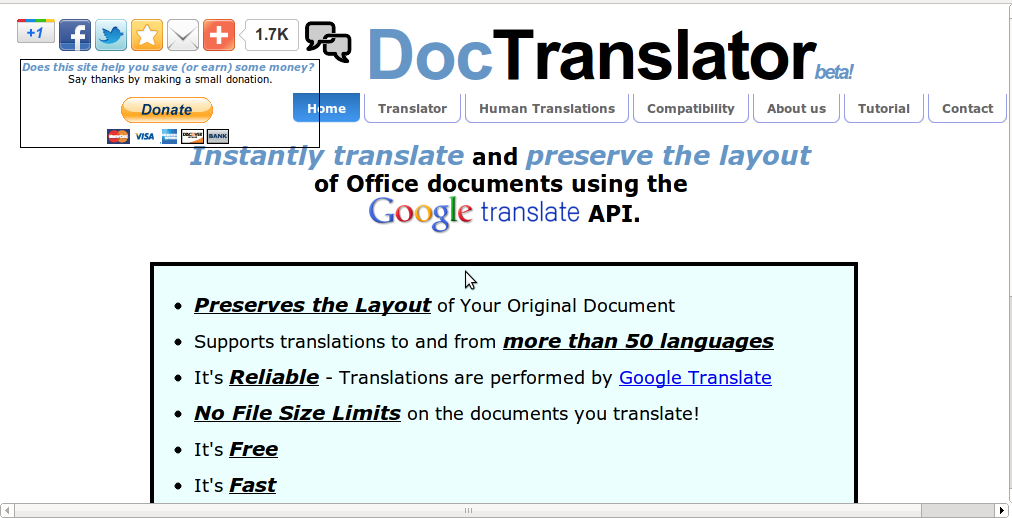
\includegraphics[scale=0.4]{ex1doctrans}
\caption{Online document translator, source: http://www.onlinedoctranslator.com/}
\end{center}
\end{figure}

From previous modules in our degree, namely Information Management 2 and Interactive Systems 3, our team had experience
of applying Jakob Nielsen's heuristics to obtain a successful user interface. We
wanted to develop the idea that our website would display the minimal amount of
information to a user by providing the registration, document upload and
language selection elements on a single page, in a simple 3 step process. Our
interface would then fall in line with the principle that user interfaces should
have an aesthetic and minimalist design.
\footnote{\url{http://www.useit.com/papers/heuristic/heuristic\_list.html}} We believe
this is an extremely important aspect of any modern website based on the way
that users make a decision of whether or not to use the services offered by the
website. For example, imagine a user enters a web-search for ``Translation
service'' and clicks our website in the results page. If the page they are met
with looks too complicated or confusing in nature, the user simply clicks
``Back'' on their web browser, and goes to the next appropriate web page. If,
however, the website looks clean, simple, and easy to use, the user would be
more inclined to investigate further. We believe that our 3-step process found on
the home page encourages anyone that requires a translation service for the
provided languages to at least try for a quote, if not go through with the whole
process.\\
\\
With this approach in mind, we began to create some wire-frames in order to form
a solid idea of how this 3-stage process would appear on our website.
\textbf{Figure 2.2} illustrates our early attempt at doing so.

\begin{figure}
\begin{center}
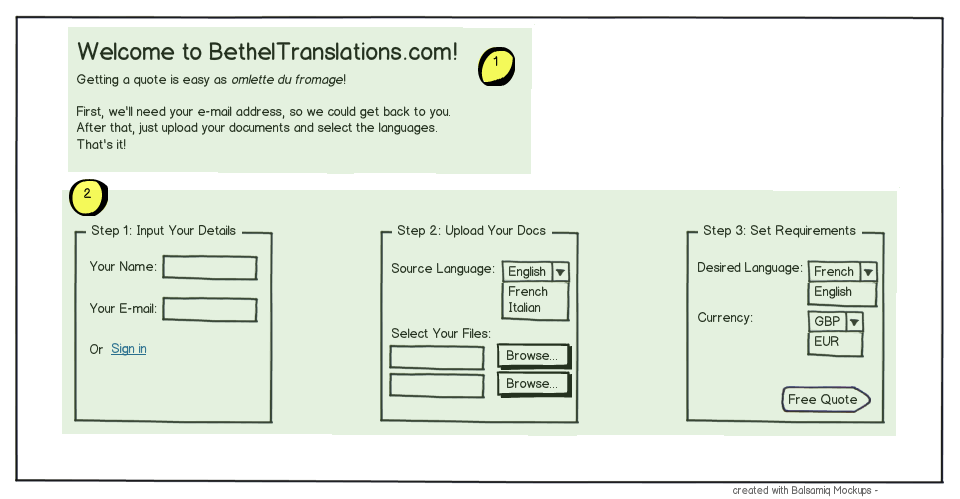
\includegraphics[width=\linewidth]{wireframes/bt-3step}
\caption{The 3-step process}
\end{center}
\end{figure}

The layout is intuitive, flowing and simple to approach. In this early design we
have divided the page into two sections. In section 1 the user is presented with
a concise block of text detailing the main functions of the site.
Subsequently, in Section 2 the user can enter their contact information, add
one of more documents, set the requirements and submit the request for a quote.\\
\\
There is no overwhelming web-form that some other websites utilise. It is minimal and
it is undemanding. The majority of the registration process happens
automatically when the user clicks ``Get your quote''. at which point the system
registers the user (pending email validation), uploads their documents to the
file store, before placing the job in
our client's pending work queue. The implementation of such functions are
discussed later in Section~\ref{chap:impl}.\\
\\


\section{User Analysis}
\label{sect:user-analysis}
With this 3-step process as our main design factor of the website, we began to
consider the main user groups of the website, identifying the needs of two
main user classes: \textbf{customer} and the \textbf{translator}

The clients are the users of the service, the visitors of the website. However,
as far as the system is concerned, not all visitors are clients, because, in
order for a visitor to become a client, he must register with the service. So we
decided to have a visitor as a category with a registered user a sub-category. A
registered user would then possess all the same abilities as a visitor with some
specialised capabilities:

\textbf{Visitor}
\begin{enumerate}
\item{Rationale: The visitor is just browsing. An anonymous visitor of the website.}
\item{Background: "I need to get some documents translated. I came across this
website and before I register or send any of my documents, I want to make sure
that I'm dealing with a serious service."}
\end{enumerate}
\begin{itemize}
\item{He/She is a potential client, therefore the steps which he must make in
order to become one must be as clear as possible.}
\item{His/Her \textbf{goal} is to inform himself/herself about the service. In
order for him/her to transition to being a customer, he/she must be convinced
that the service provided is of great quality, so the system's goal is to make
itself trustworthy. Also, a clear privacy policy regarding e-mail addresses and
the documents should be available, since they might contain sensitive data.}
\end{itemize}
\textbf{Customer}
\begin{itemize}
\item{Rationale: The customer is a registered user of the system.}
\item{He/She has the same goals as the visitor, but, now that he/she is
registered, he/she trusts the service a bit more. He/She has access to all the
documents that he/she ever submitted for translation and can view each of the
\textbf{job statuses} for which his/her documents are contained within. He/She
can view documents he/she has paid for, and up to a certain period of time,
download both the original copy and the translated copy. He/She can also view
some other useful statistics on his/her previous jobs.}
\end{itemize}
\textbf{Administrator/Translator}
\begin{itemize}
\item{Rationale: The translator is the one answering all the translation requests.}
\item{"As a translator, I must review the documents that my clients send me and
quote them. If they accept the quote, I must also translate them and let them
know when the work is complete."}
\item{His/Her goal is to answer all of the client's requests.}
\end{itemize}

\begin{figure}[h]
\label{fig:jobstatuses}
\centering
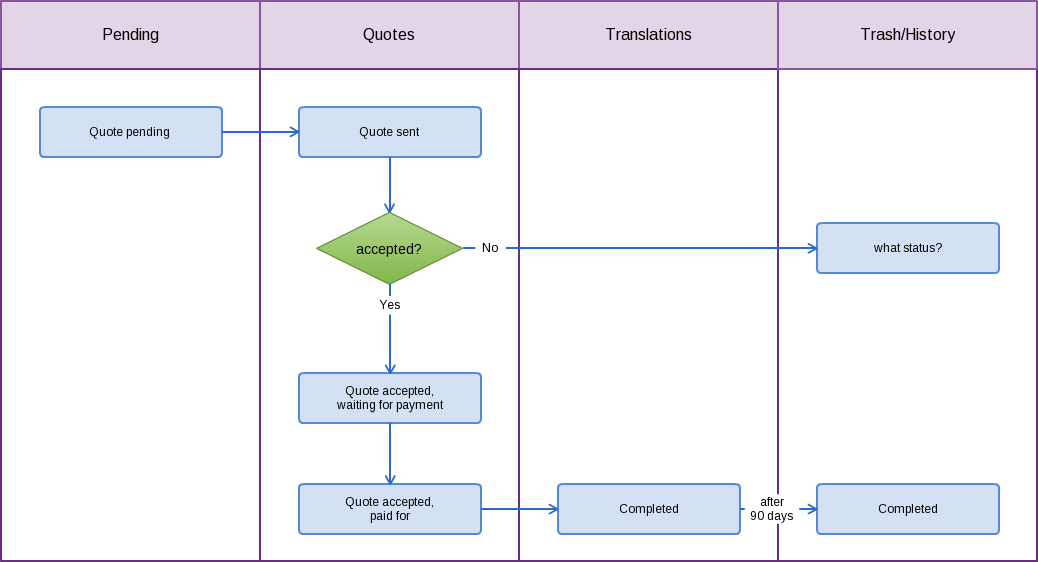
\includegraphics[width=\linewidth]{jobstatuses}
\caption{The transition of jobs through "statuses"}
\end{figure}

Building upon the needs of these user classes, we chose to design a flexible
system that provided functionality for all of these goals. Our main focal point
would be the transition of \textbf{jobs}. In the context of our system, a job is
what the website creates when the user uploads one or more documents for
translation. Clients (registered users) would submit and pay for them. The
translator would review, download the original files before uploading the
translated versions. We considered the
transition of jobs throughout the life cycle of a translation, as job statuses,
and produced a sequence that is illustrated in \textbf{Figure 2.3}. \newline

The diagram is much self-explanatory, but to summarise: Jobs that are submitted
by the clients are placed in a \textbf{pending} work queue. The translator is
able to review these documents before sending a quote to the client. After a job
has been quoted, it is placed in the \textbf{Quotes} queue. Quoted jobs are held
in this queue until they are paid for via PayPal. Once this has happened, they
are moved to \textbf{Translations}, which is a breakdown of completed jobs.
After a period of 90 days, jobs are moved to the \textbf{History}
section, the attached files being deleted permanently.\\
\\
The transformation from this design plan to a viable user interface that is
built upon these job statuses is described later in Section~\ref{sect:ui}.
\newline

\section{User Process}
\label{sect:user-process}

This section will describe the general activity flow for a client and the translator, respectively.
For the client we will try to describe the minimal stages he would likely pass through to use the 
translation service; while for the translator we will try to show his experience to finish his 
business process in a straightforward manner.

\newpage
\begin{wrapfigure}{l}{0.42\textwidth}
\vspace{-20pt}
  \begin{center}
    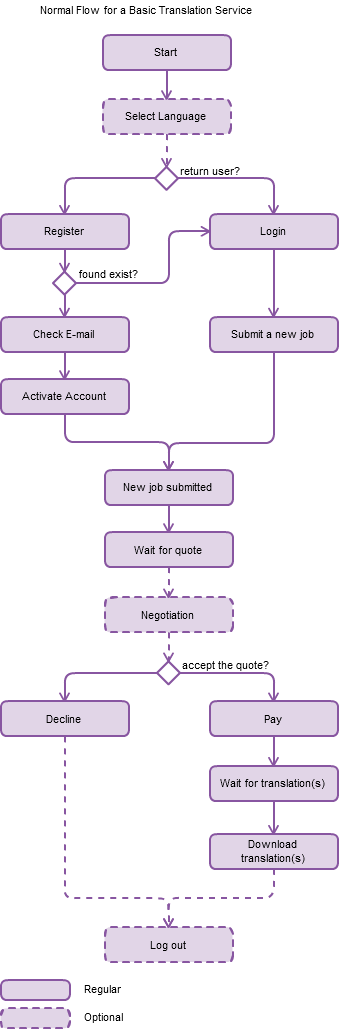
\includegraphics[width=0.4\textwidth]{images/userProcessClient.png}
  \end{center}
  \caption{userProcessClient}
\vspace{-60pt}
\end{wrapfigure}

First the client will have the option to switch among 3 displaying languages,
namely English, French and Italian. \\

To use the translation service, one must first register by: inputting name and
e-mail address, uploading one or more file(s), and setting translation
requirements (source/desire language, currency and due date). Note that
uploading is required so that only those who are actually going to use the
service are allowed to register. Also, e-mail activation is required to finish
the registration. If the system finds that the inputted E-mail address has been
registered, the client will be asked to login.\\

Either by finishing the registration process or by submitting a new job
(uploading file(s) and setting requirements) after login, a new job is
submitted.\\

Meanwhile the translator will quote the job and a negotiation on details such as
price or due date will possibly happen during this stage (it is optional,
however).\\

If the client decides to accept the quote she/he will need to pay immediately
through PayPal or could just leave it as quoted. Then the file(s) will
(hopefully) be translated by the due date and a download link of the
translation(s) will be offered in the client dashboard.\\

If the client decides to decline the offer, the translation service process will
be cancelled.\\

Other than those above, the client may: \\

	Navigate the links on the main menu: read the “About” page (information
about the service and the translator); read the “Testimonials” page; contact the
translator in the “Contact” page through the contact form; request other
services (Edit and Proofreading, Over-the-phone Interpreting and Video Remote
Interpreting) in corresponding “Service” page through the contact form. \\


\newpage

\begin{wrapfigure}{l}{0.36\textwidth}
\vspace{-20pt}
  \begin{center}
    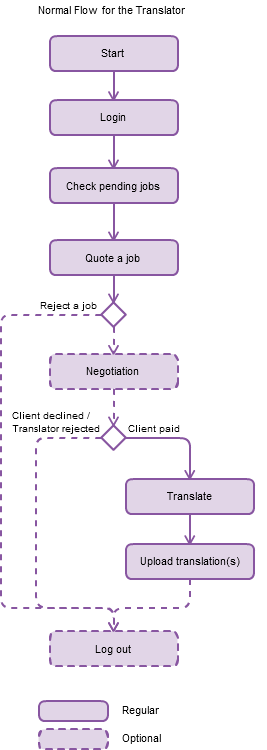
\includegraphics[width=0.34\textwidth]{images/userProcessTranslator.png}
  \end{center}
  \caption{userProcessTranslator}
\vspace{-60pt}
\end{wrapfigure}
First the translator will be directed to the admin dashboard, in which she/he
will (probably):\\

Check all pending jobs, and pick one to quote.\\ 

The quoting process will include: check the job requirements, download the files
uploaded in the job, read through the documents, set a quote and confirm it in
the dashboard. During this process, the translator may reject a job within any
stage.\\

A negotiation between the translator and a client may happen during or after the
quoting stage. They may communicate via e-mails.\\

If no rejection or declination happens, the translator will then be waiting for
the client to pay. Only after the payment is successful an actual translation
process will start.\\

Finally the translator will upload the translated documents to the server
through the admin dashboard.\\

Other than those above, the translator may: \\

Check processed jobs with different status in “Quoted”, “Accepted”, and
“Declined” sections in the admin dashboard respectively. Also all recent
translations can be downloaded through “Translations” and all past translation
records can be found in the “History” section.\\

View the statistic data for the website in “Site Statistics”.\\

	Navigate the links on the main menu: read the “About” page (information
about the service and the translator); read the “Testimonials” page.\\


\newpage
%%\rule{430pt}{1pt}

\section{Database Model}

Our database structure was designed after we had thoroughly revised our user
registration and job transition 
processes, detailed before this section. We envisaged there being four separate
entities: one for \textbf{customers} to become 
registered, one to represent \textbf{documents} being submitted, another for the
\textbf{jobs} that are comprised 
of submitted documents and finally one for the documents once they have been
\textbf{translated}. 
The attributes of each of these entities and the relationships between them is
illustrated in \textbf{Figure 2.6} 

\begin{figure}
\begin{center}
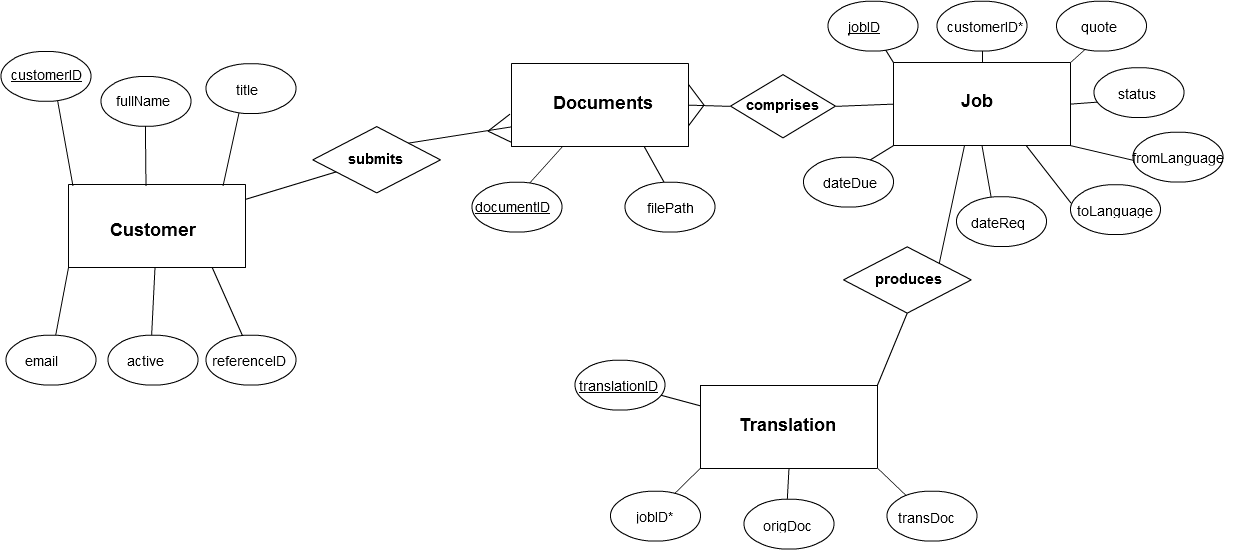
\includegraphics[scale=0.5,angle=90]{bt-erdiag}
\caption{ER Diagram for Bethel Translations}
\end{center}
\end{figure}

The majority of activity for these tables occurs in the first three entities, as
they are all populated 
in some way during the 3 stage process discussed earlier.

Discussion of the database schema, namely how we implemented the entities in the
diagram, are listed as part of Chapter \ref{chap:impl}.
% \newpage


% \newpage
\section{System Design and Wire-frames}
\label{sect:system-design-and-wireframes}
After laying out the process of the website we focused on organising the content
of the wire-frames.


\subsection{Information Architecture}
Based on the user analysis discussed in section \ref{sect:user-process}, we split
up the website into two abstract sections: 
\begin{itemize} 
	\item \textbf{Static Advertisement pages}, which are available to all visitors, and
	describe the service, means of contact, and other such information.
	\item \textbf{Dynamically generated User dashboard}, the section of the site available only to
	registered users, and which allows them to follow the progress of their translations
\end{itemize}

%TODO: maybe ``presentation'' isn't the best word to use here?
During the initial requirements capturing process, our client only offered
document translation, however during the implementation stage she obtained
certifications for other related services as well. We were now required to include pages
describing her interpreting, and proofreading services.
Since the first one is the main service, we decided that the front page of the
website would present only an overview of all of these, while focusing on the
document translation. The other services would have their own separate pages
describing them.

The main function of the \textbf{user dashboard} is to give a clear view of
the statuses of the different jobs a customer has. With the jobs life-cycle
flowchart (Figure \ref{fig:jobstatuses}) in mind, we thought that the best
approach is to have one page per status, as shown in Figure 
\ref{fig:jobstatus-page}.

\begin{figure}[h]
	\begin{center}
		%trim top bottom
		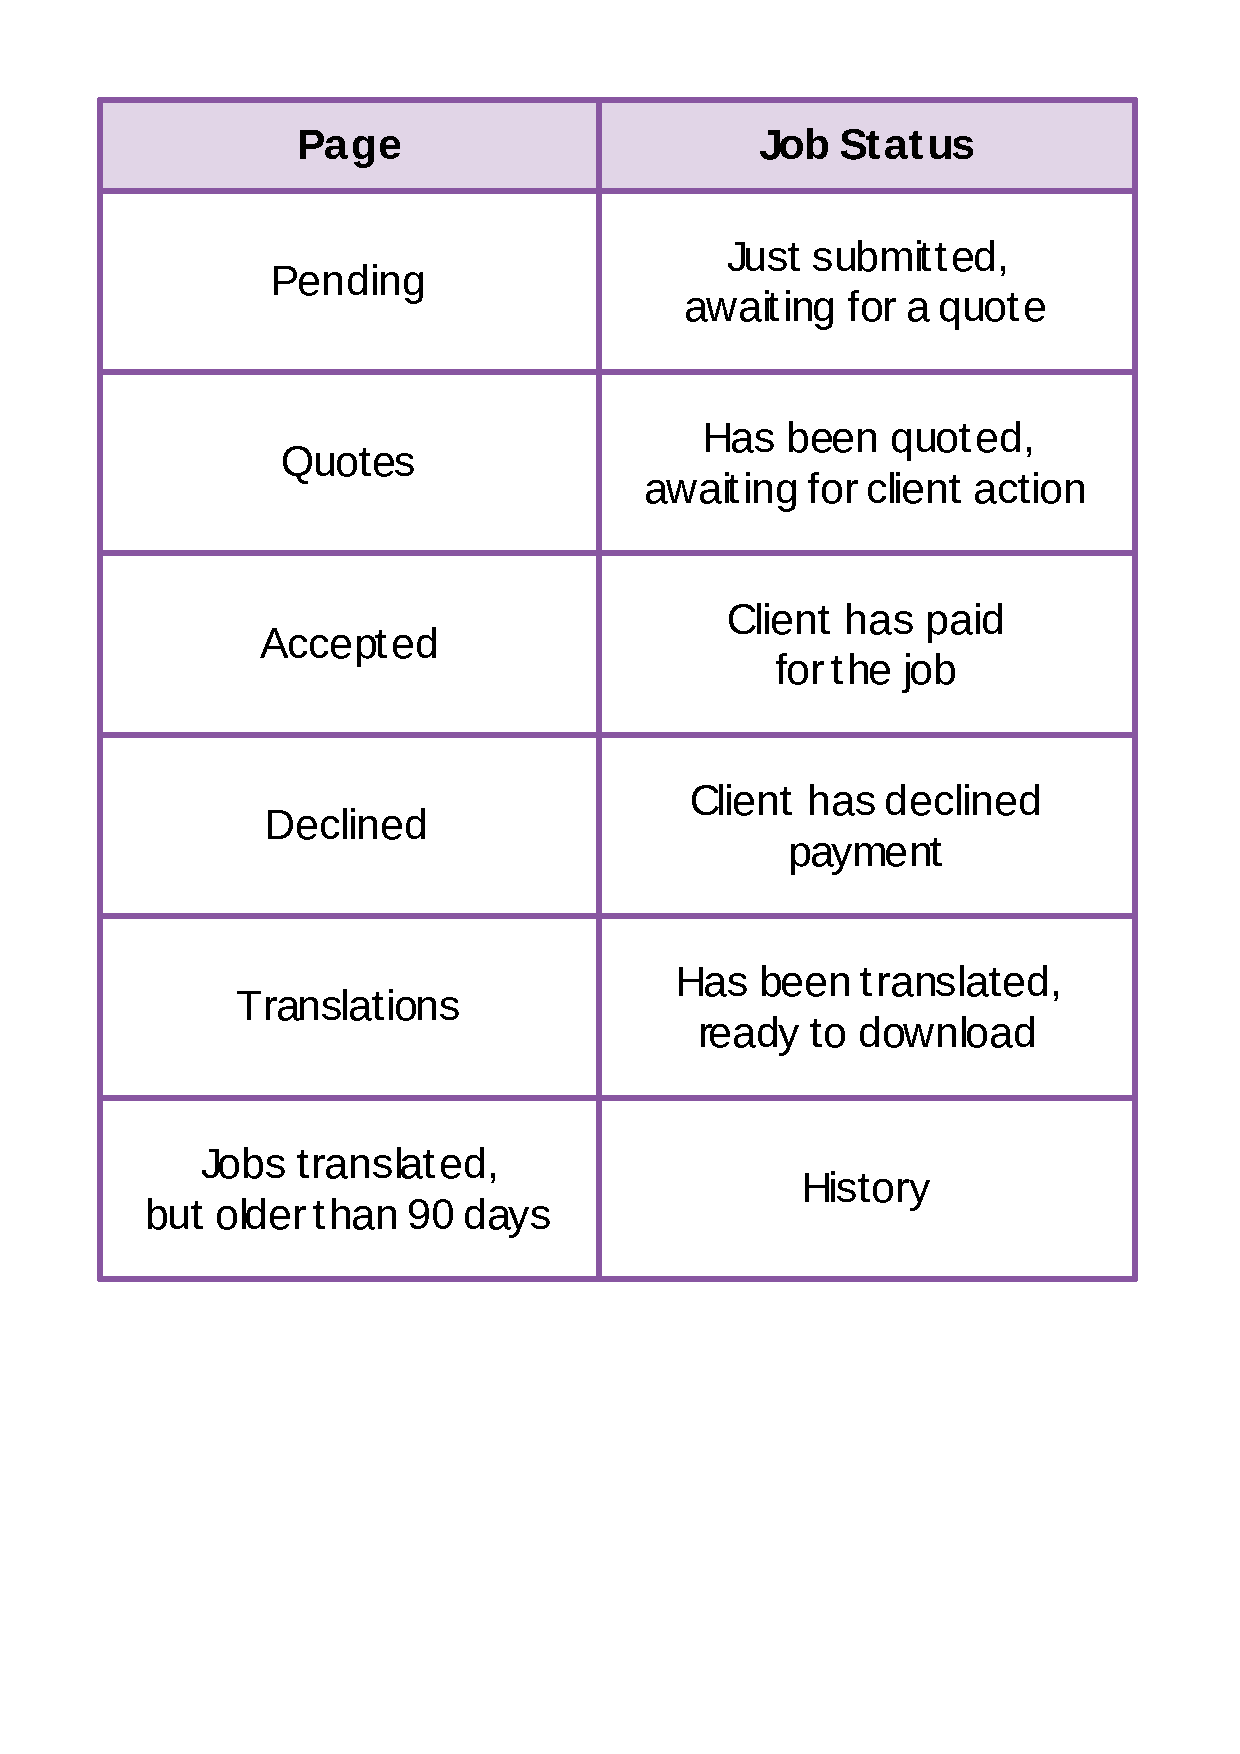
\includegraphics
			[scale=0.35, trim = 0px 150px 0px 48px, clip=true]
			{figures/jobstatus-page}
	\end{center}
	\vspace{-40pt}
	\caption{Relation between a job's status and the section of the
	dashboard it is found in.}
	\label{fig:jobstatus-page}
\end{figure}

After this evaluation, we have built a website structure diagram
(Figure ~\ref{fig:website-structure}). Everything is 1-3 clicks away.
\begin{figure}[H]
\label{fig:website-structure}
	\vspace{-20pt} %trims the whitespace on the top of the page
	\begin{center}
		\subfloat[Main]{
			%\label{fig:website-structure:main}
			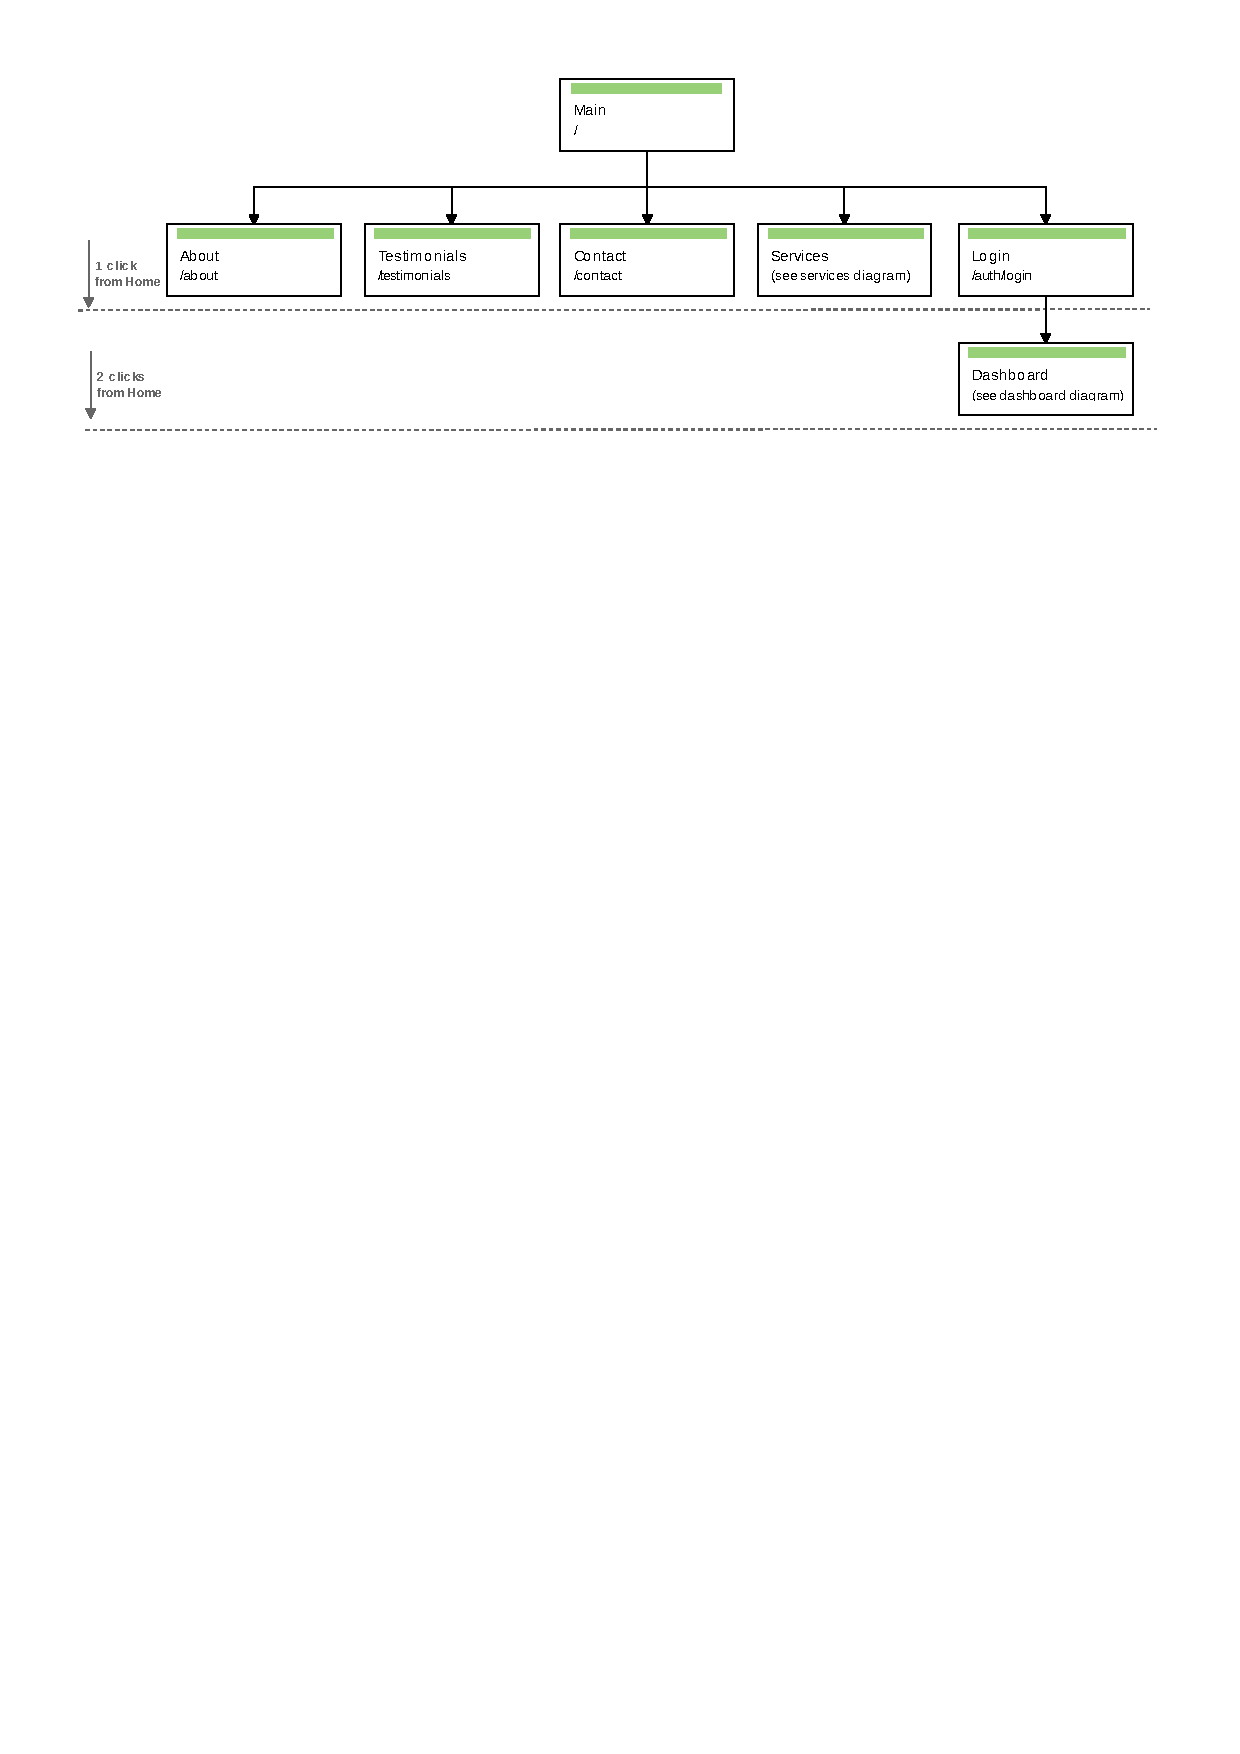
\includegraphics[
				width=\linewidth,
				% scale=0.85,
				trim=40px 600px 40px 20px,
				clip=true
				]
				{figures/website-structure}
		}
		
		\qquad
		\subfloat[Services expansion]{
			%\label{fig:website-structure:services}
			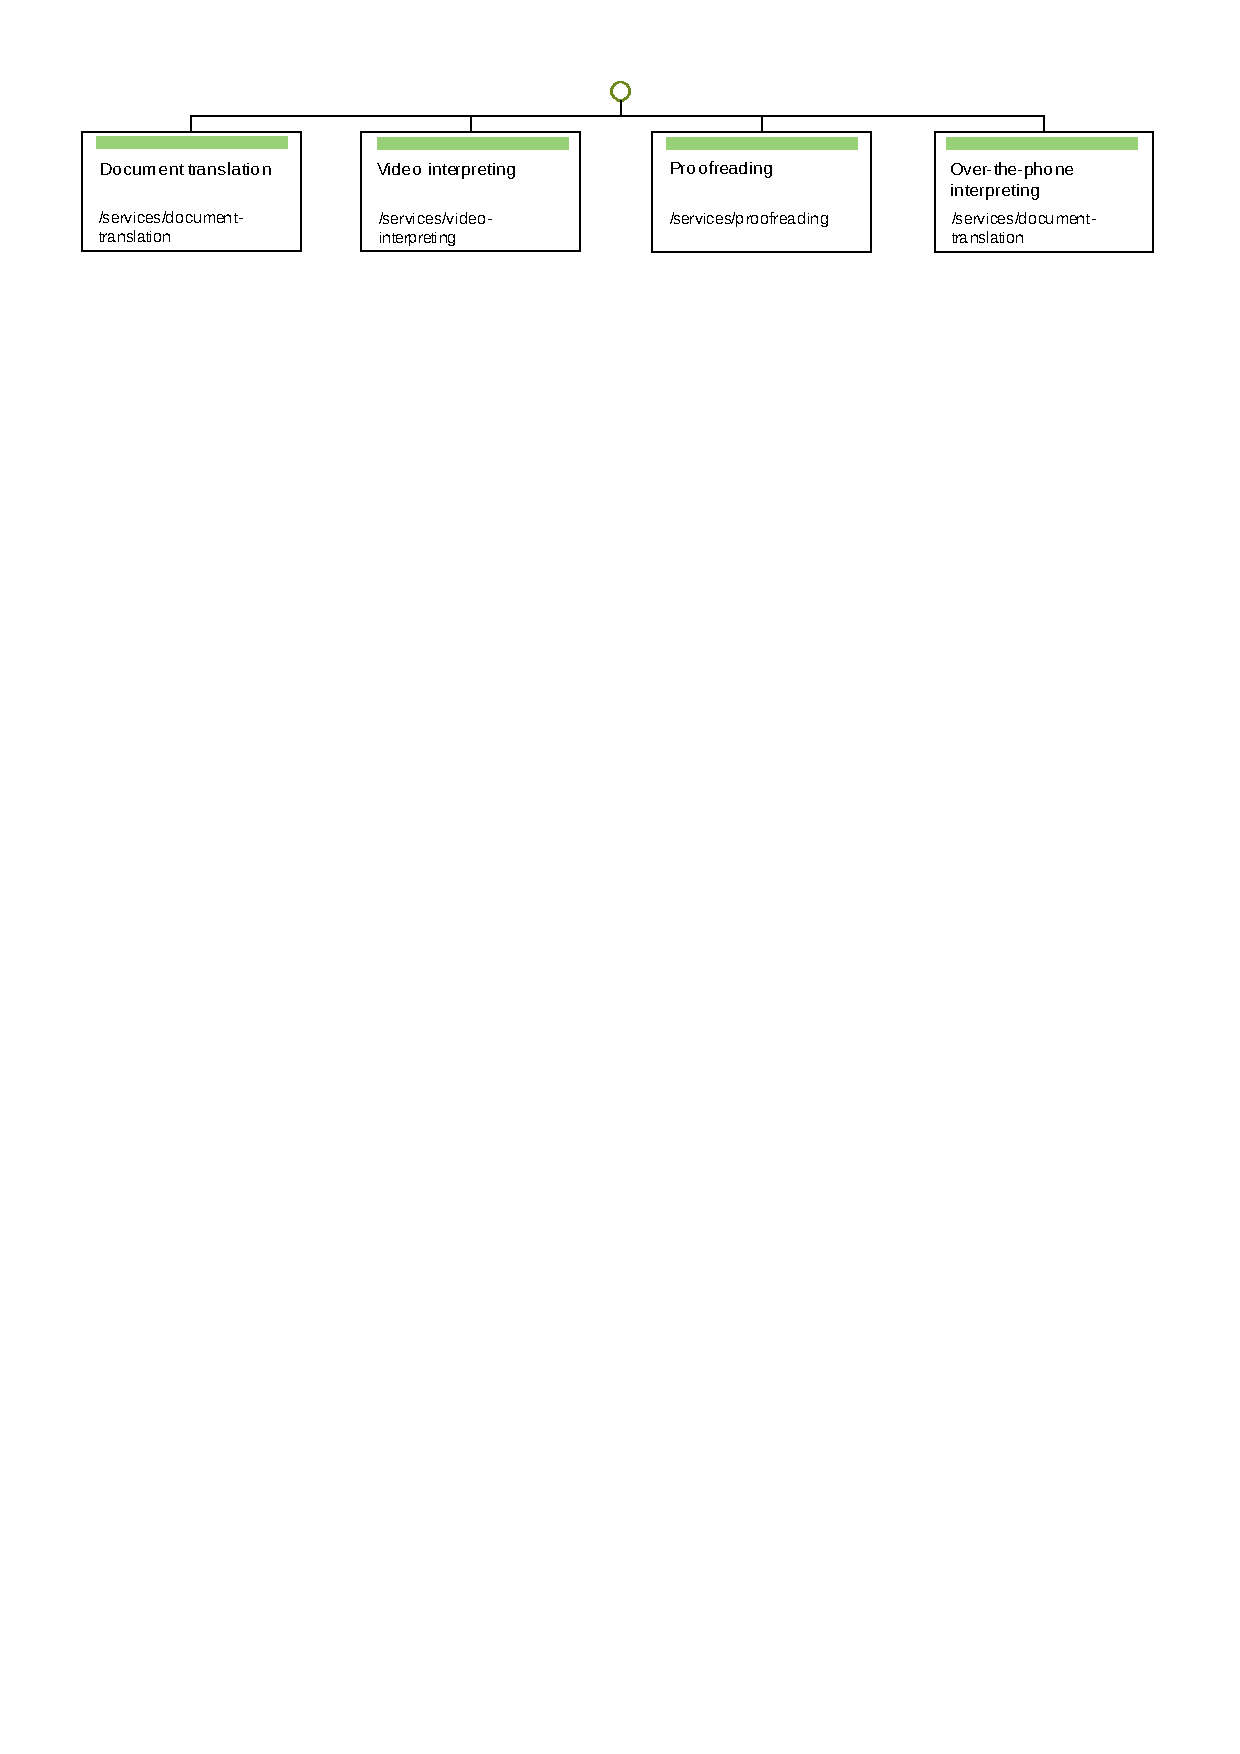
\includegraphics[
				width=\linewidth,
				% scale=0.85,
				trim=30px 700px 30px 0px,
				clip=true
				]
				{figures/website-structure-services}
		}
		
		\qquad
		\subfloat[Dashboard expansion]{
			%\label{fig:website-structure:dashboard}
			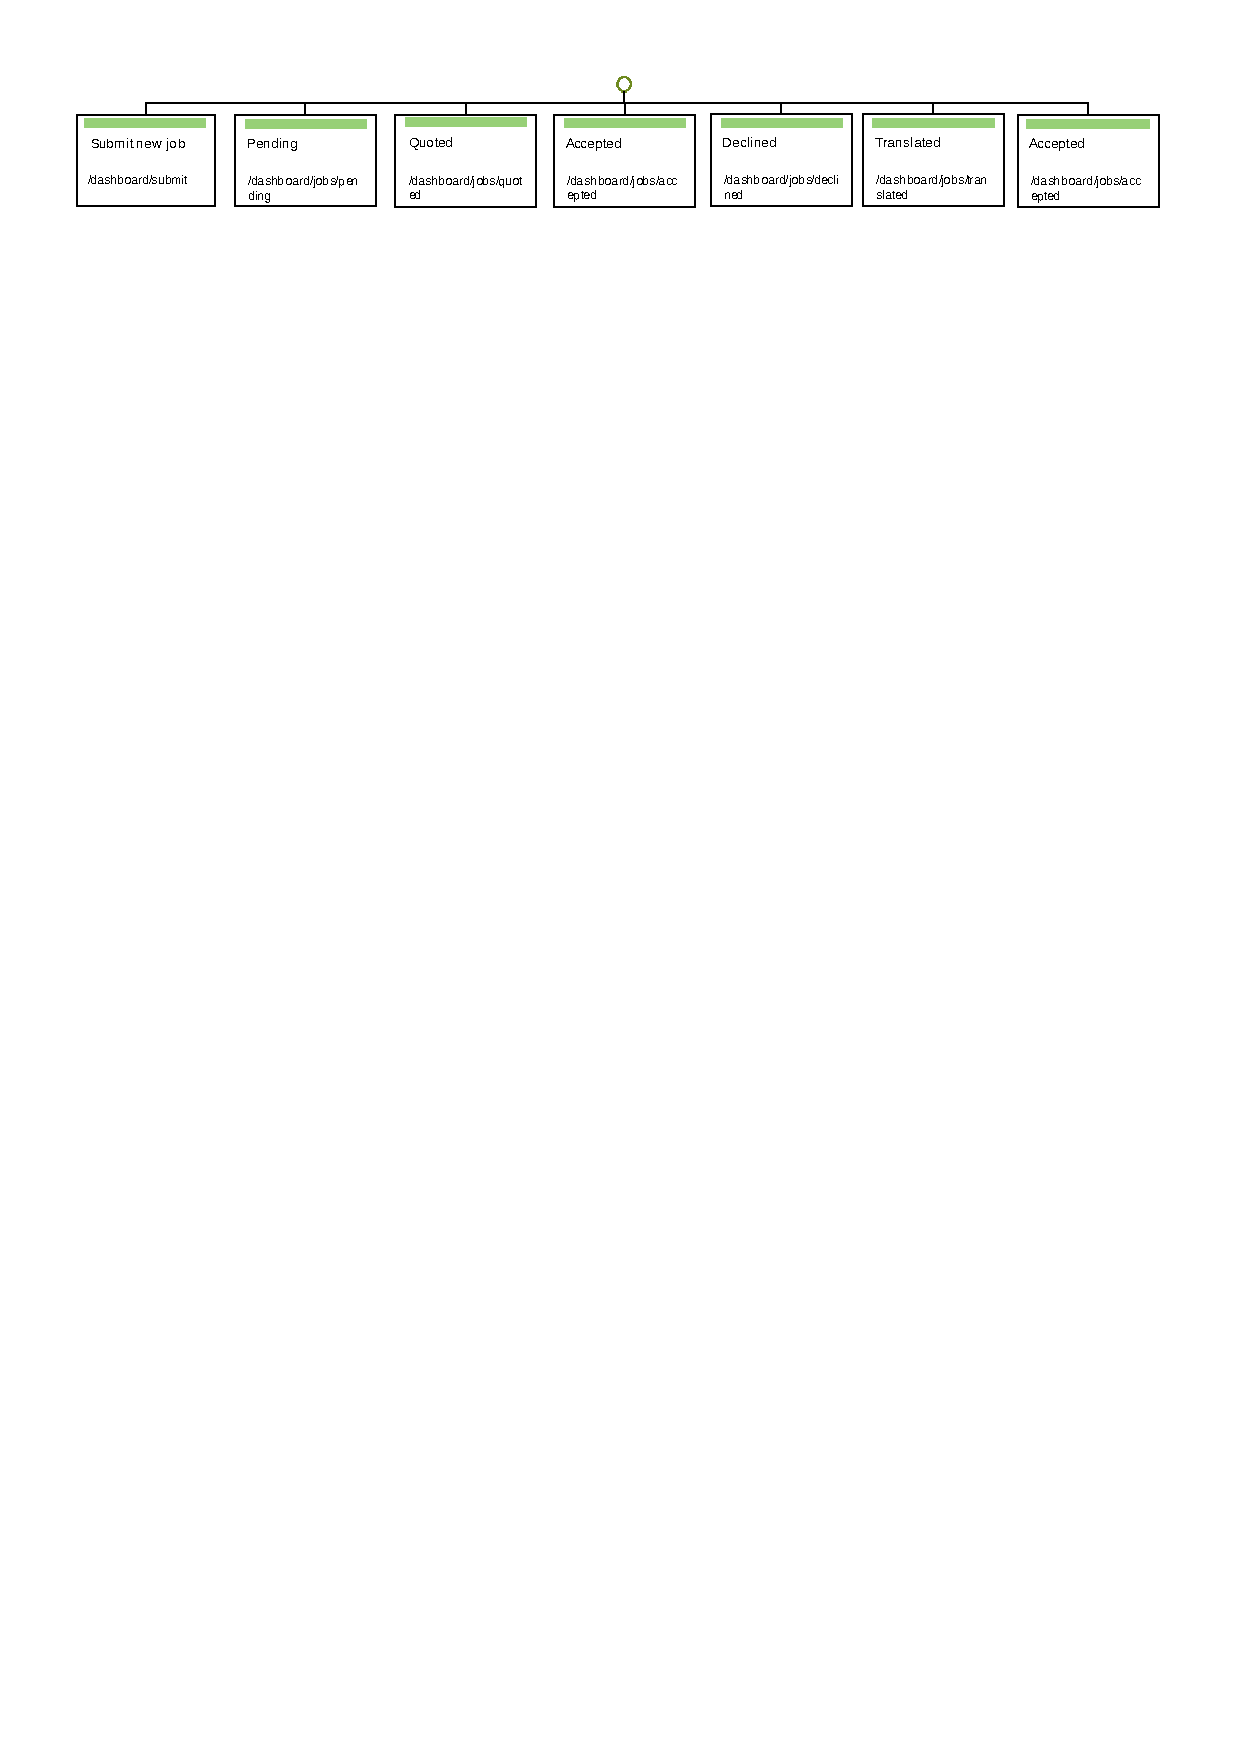
\includegraphics[
				width=\linewidth,
				% scale=0.85,
				trim=30px 700px 30px 0px,
				clip=true
				]
				{figures/website-structure-dashboard}
		}

	\end{center}
	\label{fig:website-structure}
	\vspace{-50pt}
	\caption{Website structure}
	%\vspace{-50pt}
\end{figure}

% \newpage
\subsection{Wire-frames}
% 
% paper prototypes, then functional wire-frames
% http://webstyleguide.com/wsg3/2-universal-usability/5-in-design-process.html
% 
Wire-frames are blueprints of the website, representing every important page and 
their structure and behaviour.
They focus more on what elements would a page contain, and their place on
the page, rather than a refined design. Therefore, these sketches take form of
rough drawings of the final design, avoiding specific details such as images or
colours, as they can generally distract the reader from their main purpose - is
analysing the layout of that particular page, rather than the visual design.
% some more on why these are useful, etc.


Conventions used in the wire-frames:
\begin{itemize} \itemsep1pt \parskip0pt \parsep0pt
	\item \textbf{Green background} and/or \textbf{yellow labels} - are used to
	indicate specific groups of content that will be referenced in the document.
	\item \textbf{links} - blue text and underlined
\end{itemize}

By the nature of their content, the pages can be categorised into static and
dynamic. Static pages display the same information for all users, regardless of
their status (logged in or just visiting, client or administrator). About,
Testimonials and Contact are such pages in the system described here. On the
other hand, dynamic pages draw some data from the database and display it
accordingly. In this case, the dynamic pages are the ones in the dashboard
(both client’s and administrator’s) since the information there is specific to
every client.



\subsubsection*{Template}
All the pages have this basic layout comprised of the following sections:
\begin{itemize} \itemsep1pt \parskip0pt \parsep0pt
	\item Header
	\item Content area
	\item Footer
\end{itemize}

\begin{figure}
\centering
%trim left bottom
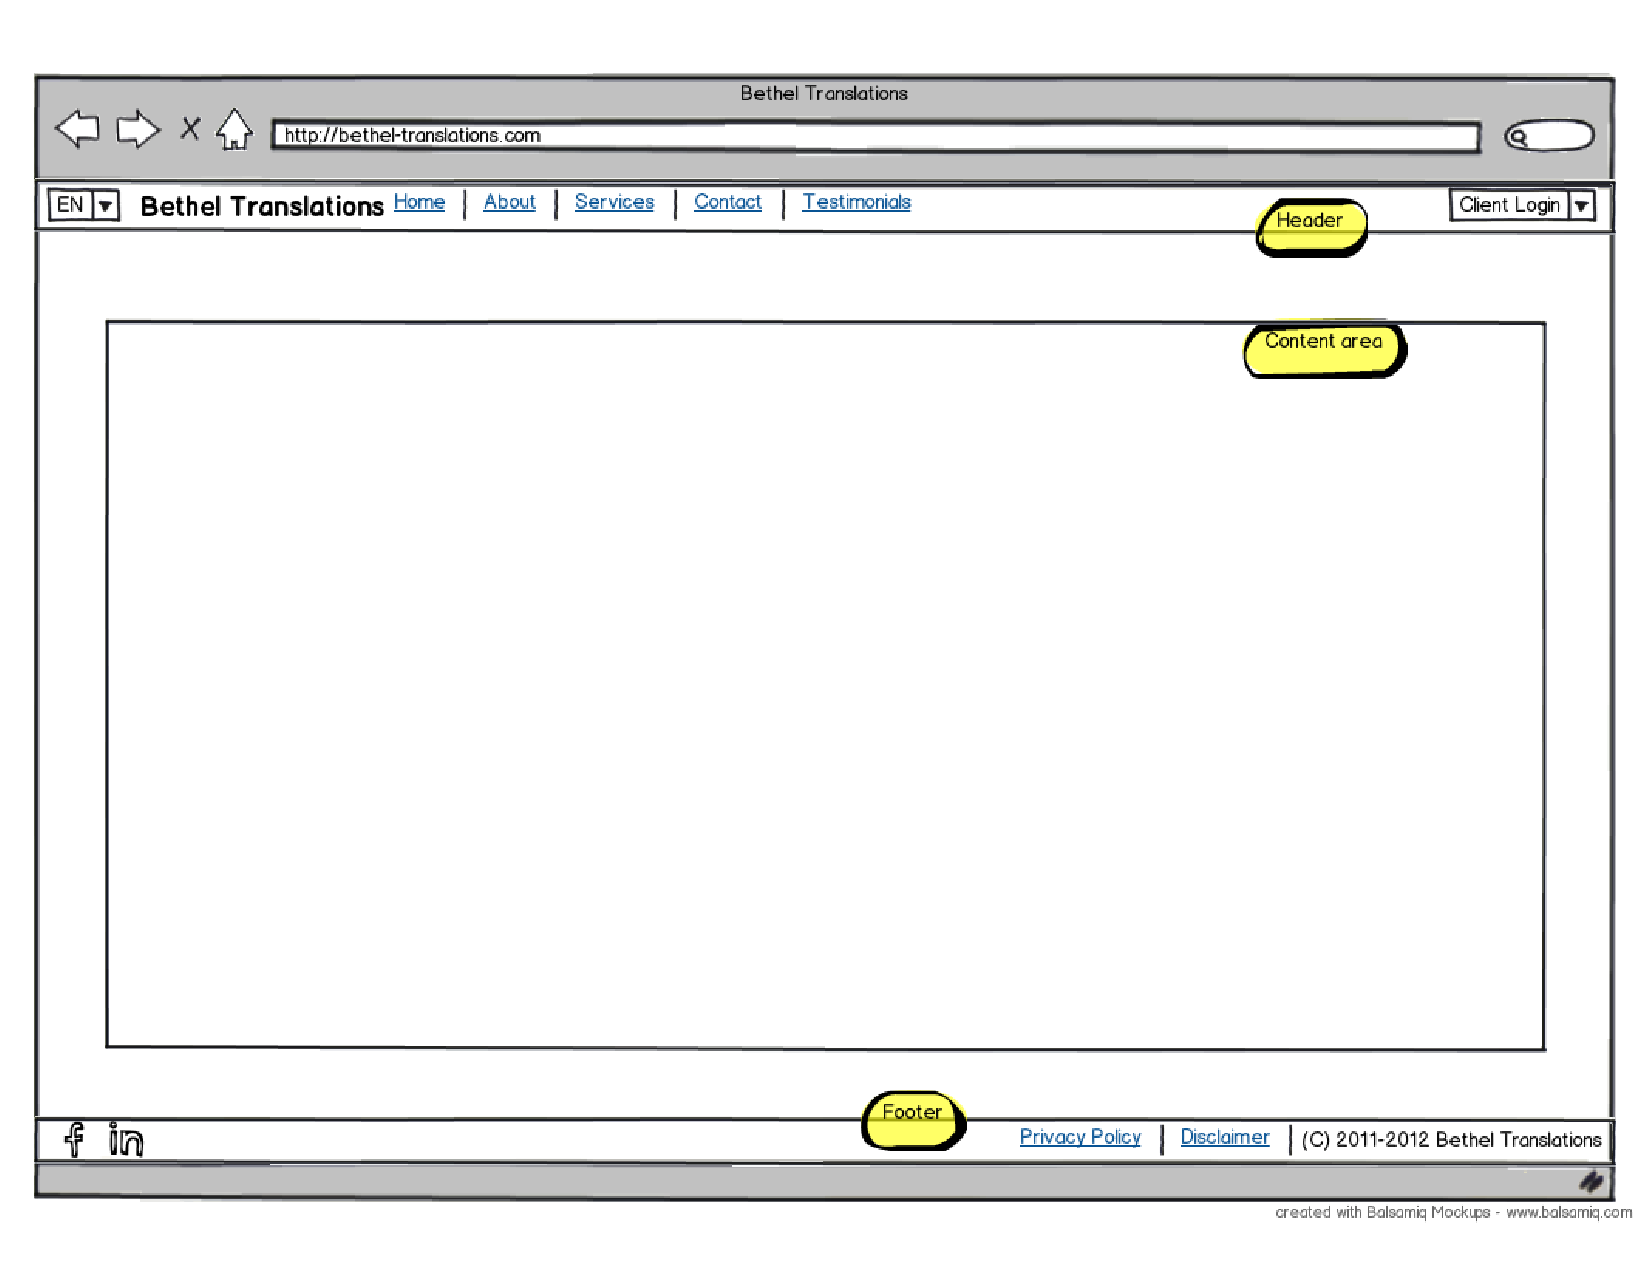
\includegraphics[width=\linewidth, trim = 0px 50px 0px 50px]
	{wireframes/main-layout}
\caption{Main layout}
\label{wireframes-main-layout}
\end{figure}

The \textbf{header} and the \textbf{footer} sections will remain unchanged
across all pages and the rest of the content goes in the \textbf{content area}.
This is a good design practice because it keeps the entire website consistent. In 
terms of technological benefits this will increase the speed of loading the website 
due to lower bandwidth requirements. The browser does not need to reload the header 
and footer every time, as it only loads the new sections. The browser will cache
these sections, improving the site's efficiency. The rest of the sketches of the pages illustrated here will only show the
content area.

The header contains:
\begin{itemize} \itemsep1pt \parskip0pt \parsep0pt
	\item \textbf{the name and/or logo of the website.} This is key as it
promotes the translators brand. Bethel Translations should be prominent to all
clients so that they know what website they are on, they can use this to recall
the services it provides and also recognise the quality of the brand at the same
time. 
	\item main navigation menu
\end{itemize}

Within the pages, primary navigation is provided on the top of the
screen, in a horizontal list of text links. In the dashboard navigation is
provided on the left, in a vertical list of text links.
\begin{itemize} \itemsep1pt \parskip0pt \parsep0pt
	\item Home
	\item About
	\item Services
	\item Testimonials
	\item Contact
	\item Login - this link must stand out, since it is of a higher
	importance and the page linked is of a different nature than the rest,
	so it is separated from the others.
\end{itemize}


Footer:
\begin{itemize} \itemsep1pt \parskip0pt \parsep0pt
	\item copyright notice, if needed
	\item links to legal documents (e.g.: Privacy policy, terms of use, etc)
	\item awards or certifications (translation services related, 
	PayPal certification)
	\item contact information (actual information or just a link to the 
	`Contact’ page)
	\item link to the business’ Facebook page
\end{itemize}
% end of Template


\subsubsection{Main page}
From our earlier decision of creating a simple three step process and
implementing this on our homepage, we took our wire-frame and refined it to
come up with the  \textbf{Main Template} (Figure ~\ref{wireframes-main-layout}).

\begin{figure}[ht]
\label{wireframes:main-template}
\begin{center}
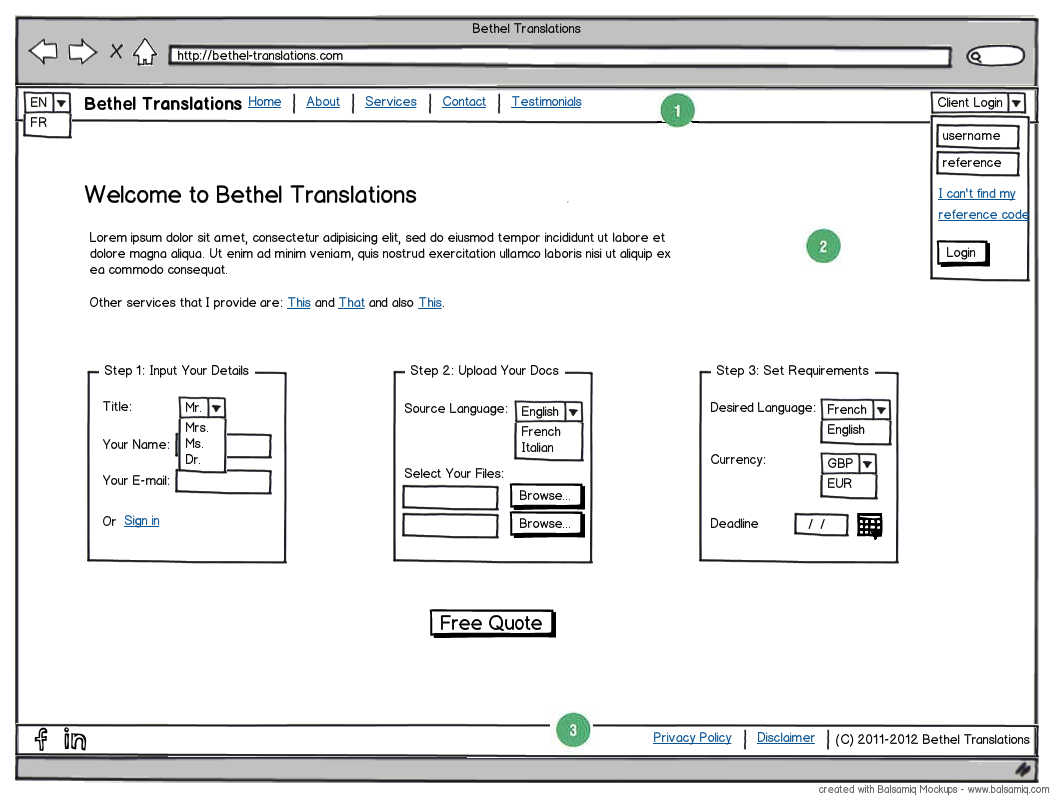
\includegraphics[width=\linewidth]{wireframes/bt-homepagev3}
\caption{The Main Template}
\end{center}
\end{figure}

The site-wide header (labelled 1) and footer (labelled 3) can clearly be seen to
be simple and uncluttered.
% end Main page


\subsubsection{About}
This is the page the users would go to in order to find out more about the
service. Contains a few paragraphs that detail goals and accomplishments.
The page needs to answer some possible questions that the users might have
regarding the business:
\begin{itemize}
	\item Who is behind it?
	\item What are they doing?
	\item When did they start doing it?
	\item Where are they?
	\item How are they accomplishing what they claim to do?
	\item Optionally an image, or even a short video, to enhance trustworthiness.
\end{itemize}

\begin{figure}
\label{wireframes:about}
\begin{center}
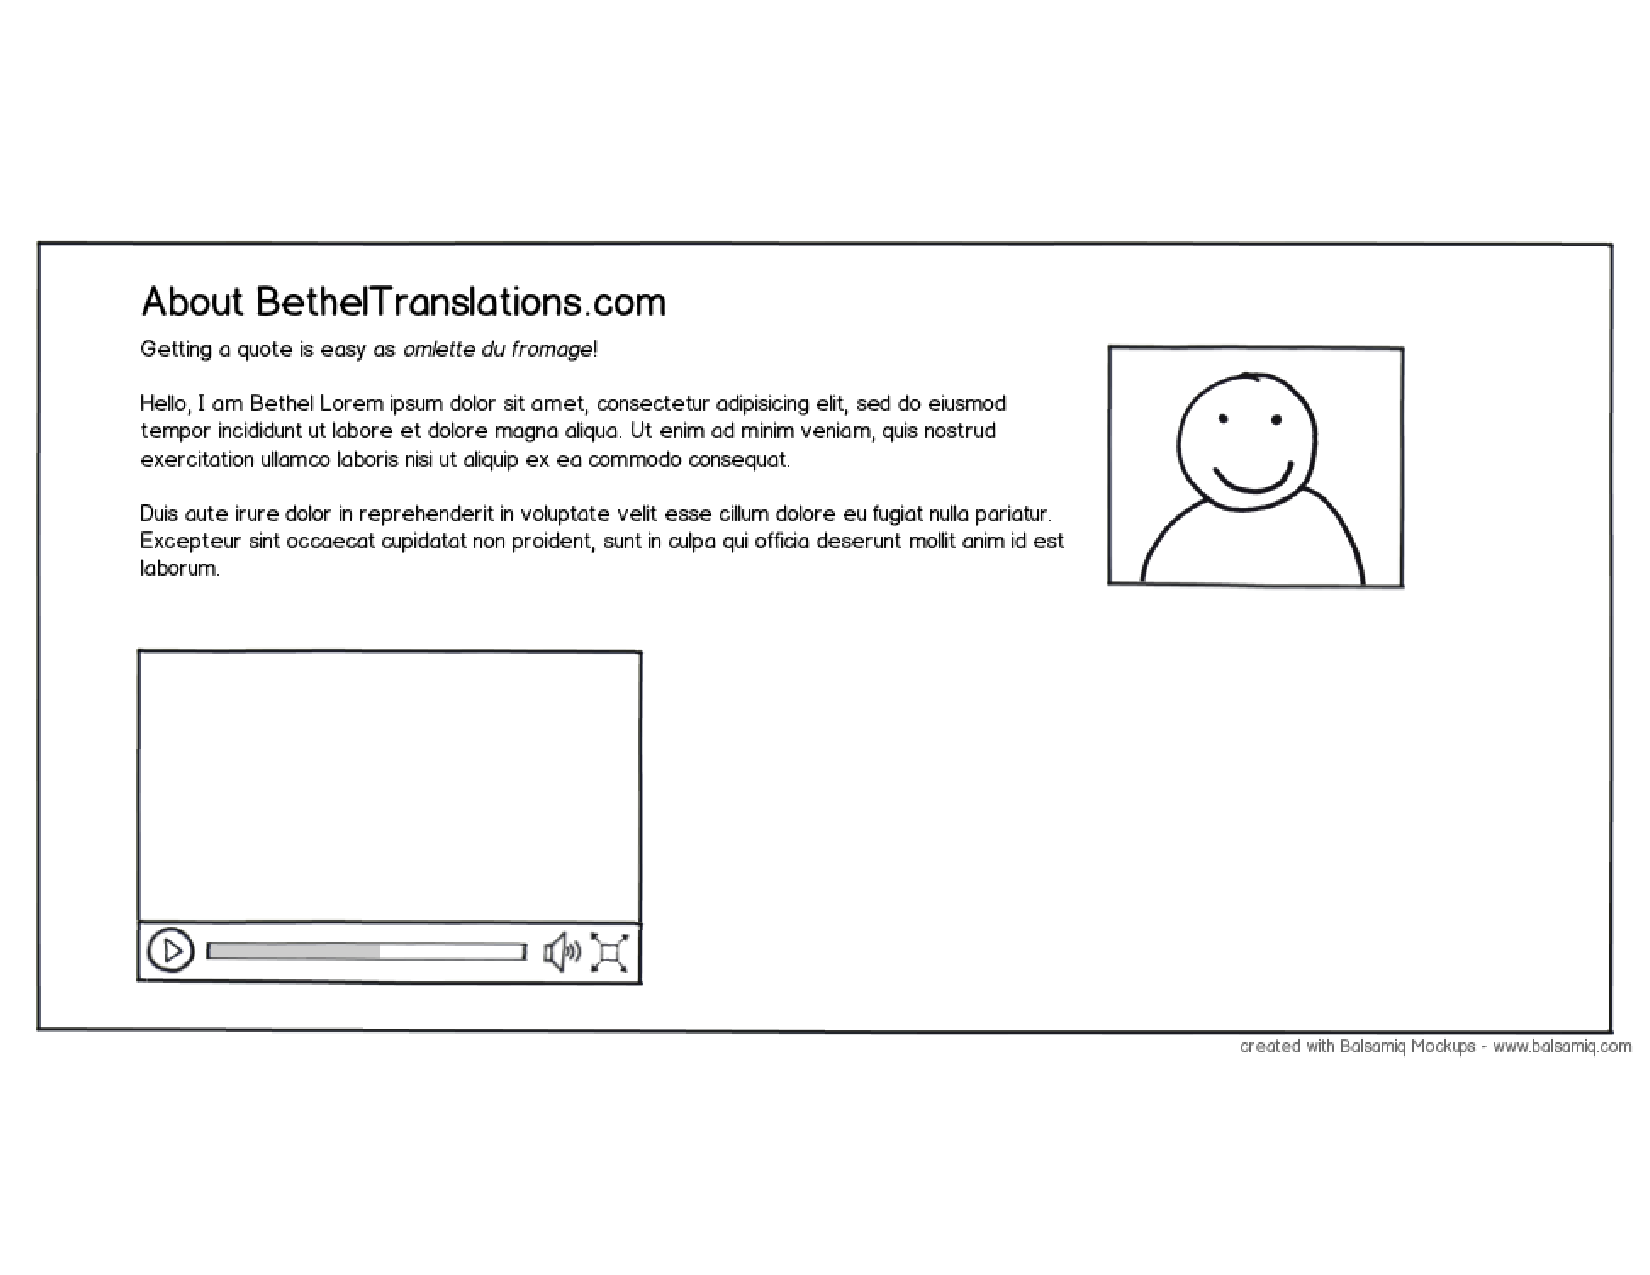
\includegraphics[width=\linewidth, trim = 0px 110px 0px 100px]{wireframes/about}
\caption{The About page}
\end{center}
\end{figure}
% end About


\subsubsection{Testimonials}
Testimonials from happy customers will likely add to the level of trust
prospective customers have with this business.
The business owner would ask her clients for feedback and permission to publish
it on the website. Then she can pick which ones would suit her and post only a
fragment on the website, along with some details of that client (name, company,
occupation).

\begin{figure}
\label{wireframes:testimonials}
\begin{center}
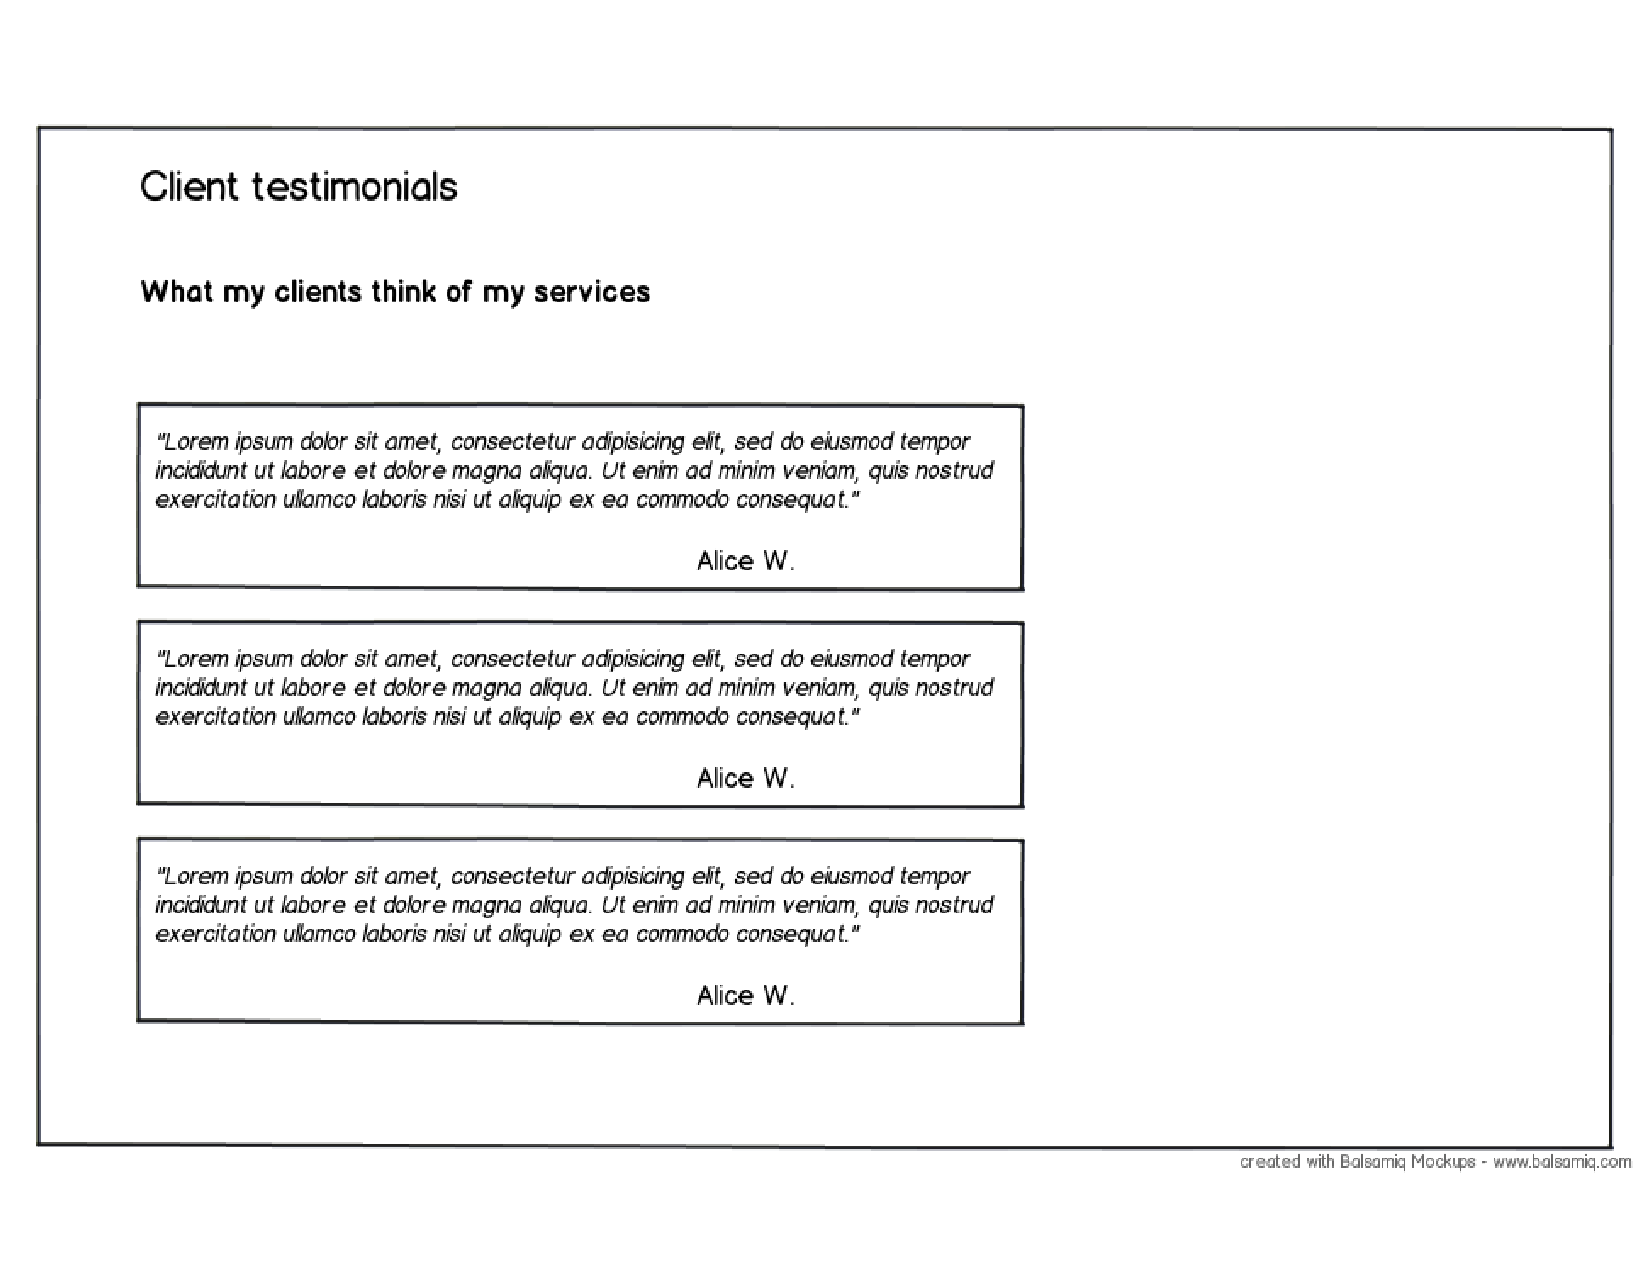
\includegraphics[width=\linewidth, trim = 0px 80px 0px 220px]
	{wireframes/testimonials}
\caption{The Testimonials page}
\end{center}
\end{figure}
% end Testimonials


\subsubsection{Contact}
Having other contact methods (phone number, physical mailing address) also add
to the credibility of the business. ``A company with no address is not one you
want to give money to.'' [Jakob Nielsen]
\begin{enumerate} \itemsep1pt \parskip0pt \parsep0pt
	\item work telephone number
	\item physical address
	\item social media pages
	\item contact form (by e-mail)
\end{enumerate}

\begin{figure}
\label{wireframes:contact}
\begin{center}
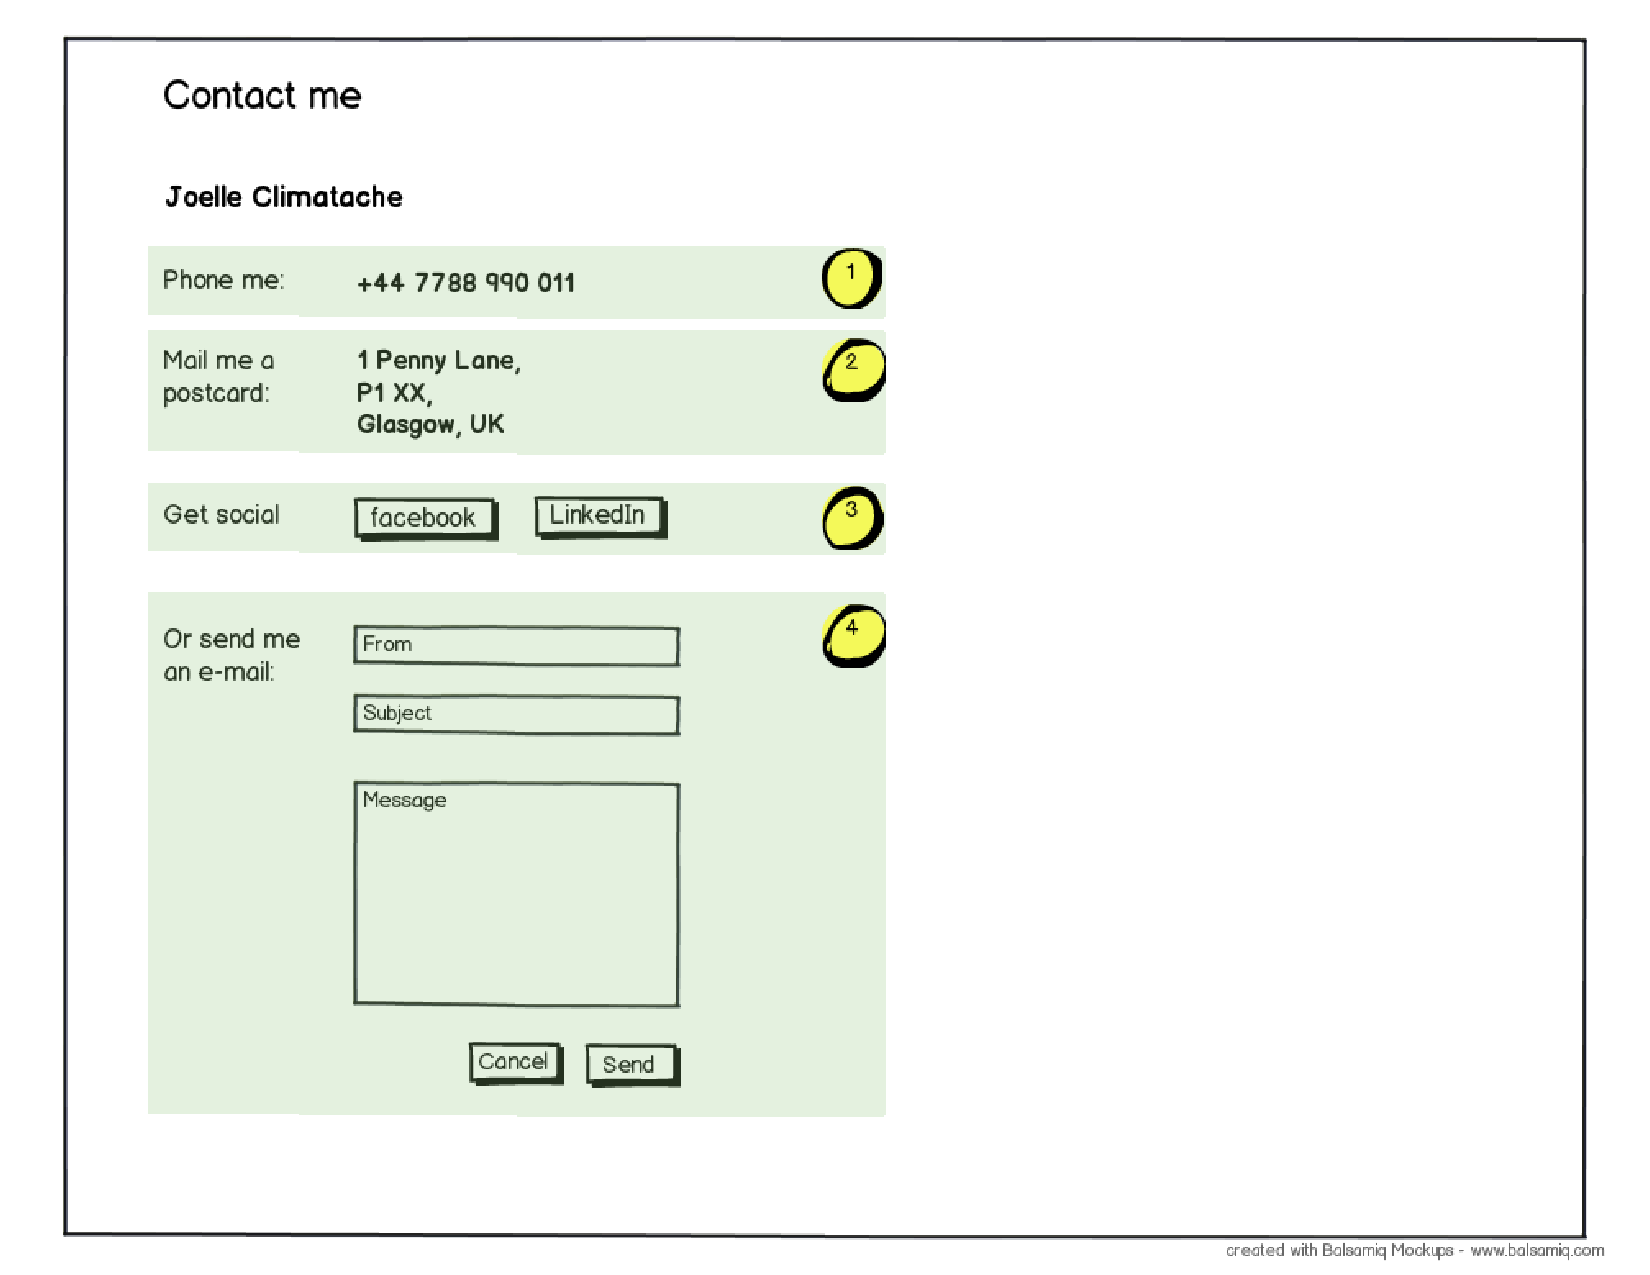
\includegraphics[width=\linewidth, trim = 0px 40px 0px 220px]
	{wireframes/contact}
\caption{The Contact page}
\end{center}
\end{figure}
% end Testimonials

\subsection{Summary}
From the images and diagrams in this chapter we have constructed the blueprints
for a modern, stylish, and most significantly - user friendly website.
Ultimately the website we want to build is one the client can fully use, without
any reluctance. The next chapter, \ref{chap:impl}, describes how we transitioned
from design to implementation, and the methods used in doing so.

%==============================================================================
\chapter{Implementation}
\label{chap:impl}

In this chapter, we describe how we implemented the system from our design plan
and detail the technologies used in doing so.

%------------------------------------------------------------------------------

\section{Development Environment}
\label{sect:dev-env}
Bethel Translations, like all modern websites, makes use of multiple
technologies in order to provide both the rich user interface and the handling
of the various background operations which are integral to a system such as this.
These two distinct entities form part of the client/server
model\footnote{\url{http://en.wikipedia.org/wiki/Client-server\_model}}.\\
\\
Utilising this model for our design, the client domain includes all of the programming code which runs in the
user's web browser, whilst the server domain encompasses the logical operations
performed on the web server.\\
\\
Programming for the project was split between several web-orientated languages.
The central development language was PHP for developing the controllers and
models. HTML5, JavaScript and jQuery were used in the views. As mentioned
previously we employed the use of two frameworks, namely CodeIgniter and
TankAuth. CodeIgniter provided the Model-View-Controller architecture PHP
framework for the website, and TankAuth is an open source authentication library
for CodeIgniter.\newline
\newline
As we learned from the Distributed Information Management course we studied this
year, web-development is ever-changing and to stay current developers must adapt
to using new technology. As a result of this we have coded the views using the
newest HTML5 standard. This will allow future developers to maintain the site
with ease as adding new modern features will be simpler.\newline
\newline
Another thing we learnt from our Distributed Information Management course is
that it is desirable to separate out our concerns when developing in a web
environment. This led us to using the open source Twitter Bootstrap
\footnote{\url{http://twitter.github.com/bootstrap/}}. Bootstrap is ``simple and
flexible HTML, CSS, and JavaScript for popular user interface components and
interactions''. During the implementation stage, Twitter released an upgraded version,
version 2.0, of Bootstrap and we upgraded to this version when it was released
in early 2012.\newline
\newline
For implementation purposes we set up an online
SVN using Google Code. This version control system allowed us to keep track of
changes, report and resolve issues, and maintain a wiki of useful pieces of
information that we needed to keep and track.\newline
\newline Further to this we also set up a test server to allow us to view our site live on the web as we
developed it and to test any changes as we made them.\newline
\newline

\section{Prototype} \label{sect:proto}
One of the many benefits of the client/server model is the opportunity to
completely separate development of the user interface from the background
processes. 
We were able to quickly implement a mockup of the interfaces, while not worrying
about the actual processes which would happen behind the scenes. A static
representation of the design for the site was developed in order to allow our
client to see early on exactly how the site would look and operate once it was
fully operational.

\section{User Interface} \label{sect:ui} 

This section aims to show the user interface of our final product. 
From the structure to the navigation and finally the description of all the main pages.

\subsection{Structure and Navigation}

The overall structure of the application is relatively simple, as shown 
in the website structure diagram (Figure ~\ref{fig:website-structure}). 
Everything is 1 to 3 clicks away.

\textbf{Navigation}

Pages are displayed in a single browser window, with the exception
of some modal windows that hover over the main page to show notifications. The modals
contain no browser controls. Links are provided to close them.

\subsection{Page Descriptions}

This major part of the document contains detailed descriptions of
each screen from the Bethel Translations website.

Some of the similar pages are omitted in order to avoid redundancy.

\textbf{Welcome Page}
\begin{figure}[H]
\centering
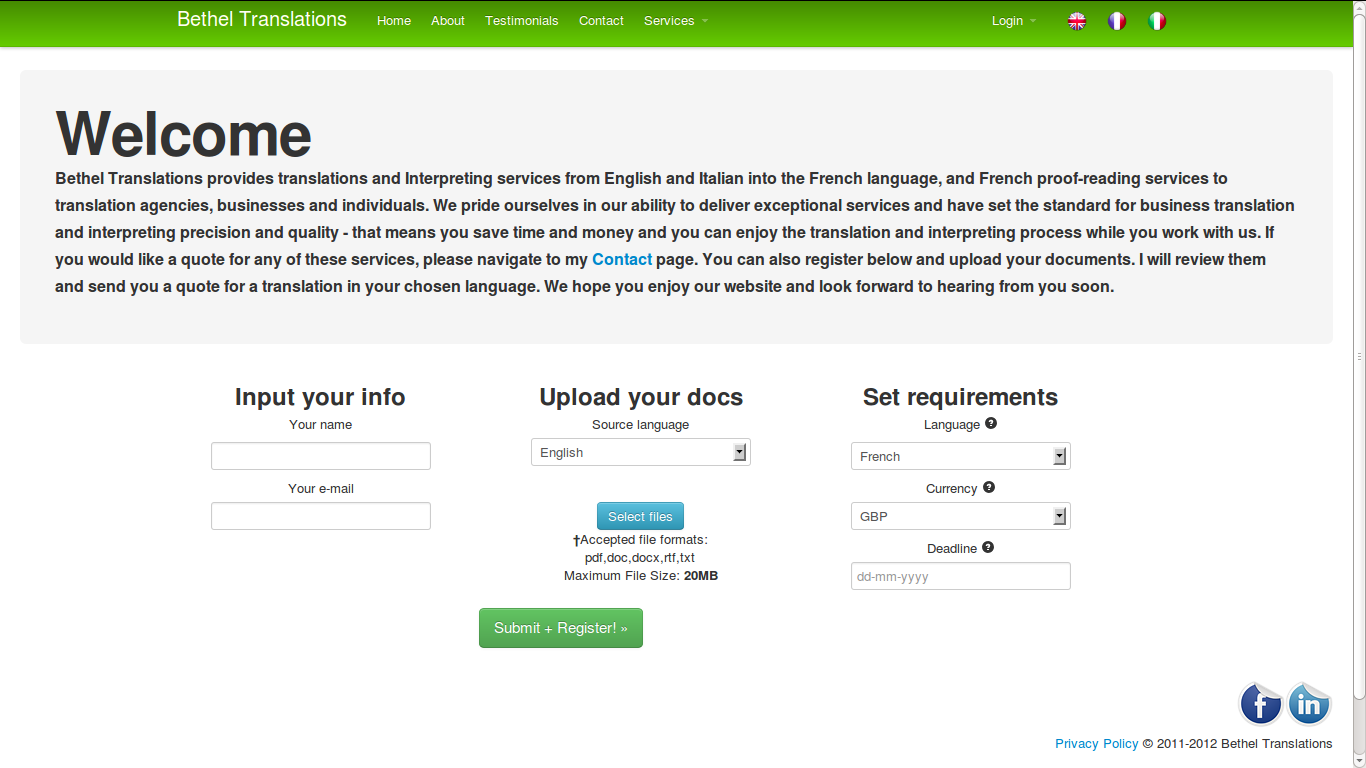
\includegraphics[width=0.8\linewidth]{images/welcomePage}
\vspace{-30pt}
\end{figure}

\begin{itemize}
\item \textbf{Description}

This is the landing page of the website. 

\item \textbf{Navigation}

This is the default page a potential customer will see when visiting the website. One can always come back to this page with the text link ``Home".
However, the registration process will not be shown for a logged-in user. Instead, they will see a message that directs them to the dashboard to submit new jobs.

\item \textbf{Main Elements}
\begin{itemize}
\item `Main Menu Bar'\\
Type: Text links\\
Content: Links to the About page, the Testimonials page, the Contact page, and the Service pages. Links to versions of the website in different languages. \\
Behaviour: The user is directed to the destination of a particular link. \\

\item `Login' / `My Account'\\
Type: Drop-down box\\
Content: (For `Login') Fields `Email' and `Password' to input login information; check-box `Remember me' to provide cookie feature; 
text link `Forgot password' directing to password resetting process. (For `My Account') text links `Dashboard' and `Logout'.\\
Behaviour: `Login' is shown by default. `My Account' is shown for a logged-in user.\\

\item `Register'\\
Type: Field\\
Content: Fields to input registration information and job requirements; button to upload files; 
button to register and submit a new job request (this request will only be presented to the translator after the user activates his account).\\
Behaviour: Disappears after a user logged in. A modal telling the user to activate his account will pop up when submitting. \\
\end{itemize}
\end{itemize}

\textbf{Contact Page}
\begin{figure}[H]
\centering
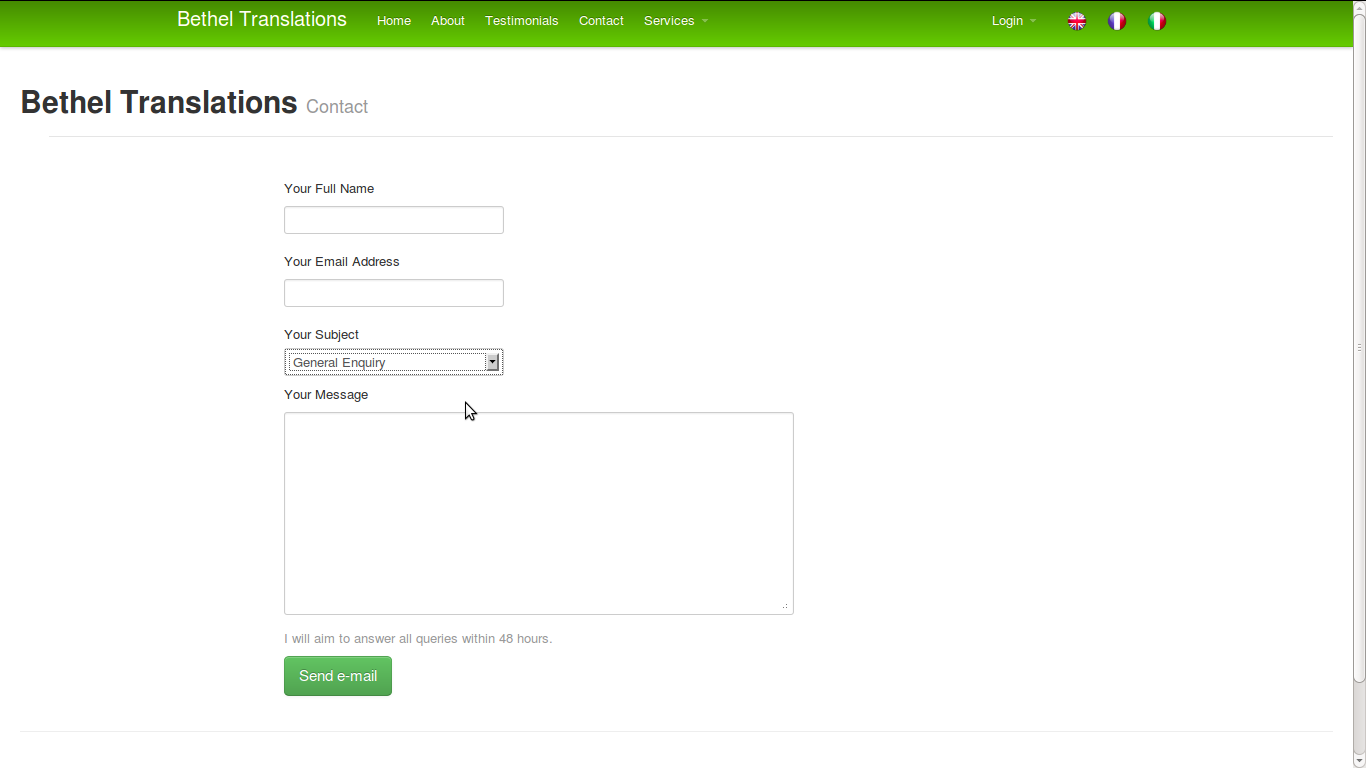
\includegraphics[width=0.8\linewidth]{images/contactPage}
\vspace{-30pt}
\end{figure}

\begin{itemize}
\item \textbf{Description}

The contact page is the page that a customer may use to contact the translator for general enquiries or getting a quote for services other than document translating that the translator offers. 

\item \textbf{Navigation}

A user can get access to this page through the text link `Contact' on the main menu bar.

\item \textbf{Main Elements}
\begin{itemize}
\item `Contact Form'\\
Type: Form\\
Content: Text fields to input user information; drop-down box to choose a enquiry subject; text field to leave messages to the translator. \\
Behaviour: Full name and email address will be automatically filled for a logged-in user. An enquiry email will be sent to the translator. \\

\end{itemize}
\end{itemize}

\textbf{Administrator Dashboard - Pending/Quoted Jobs}
\begin{figure}[H]
\centering
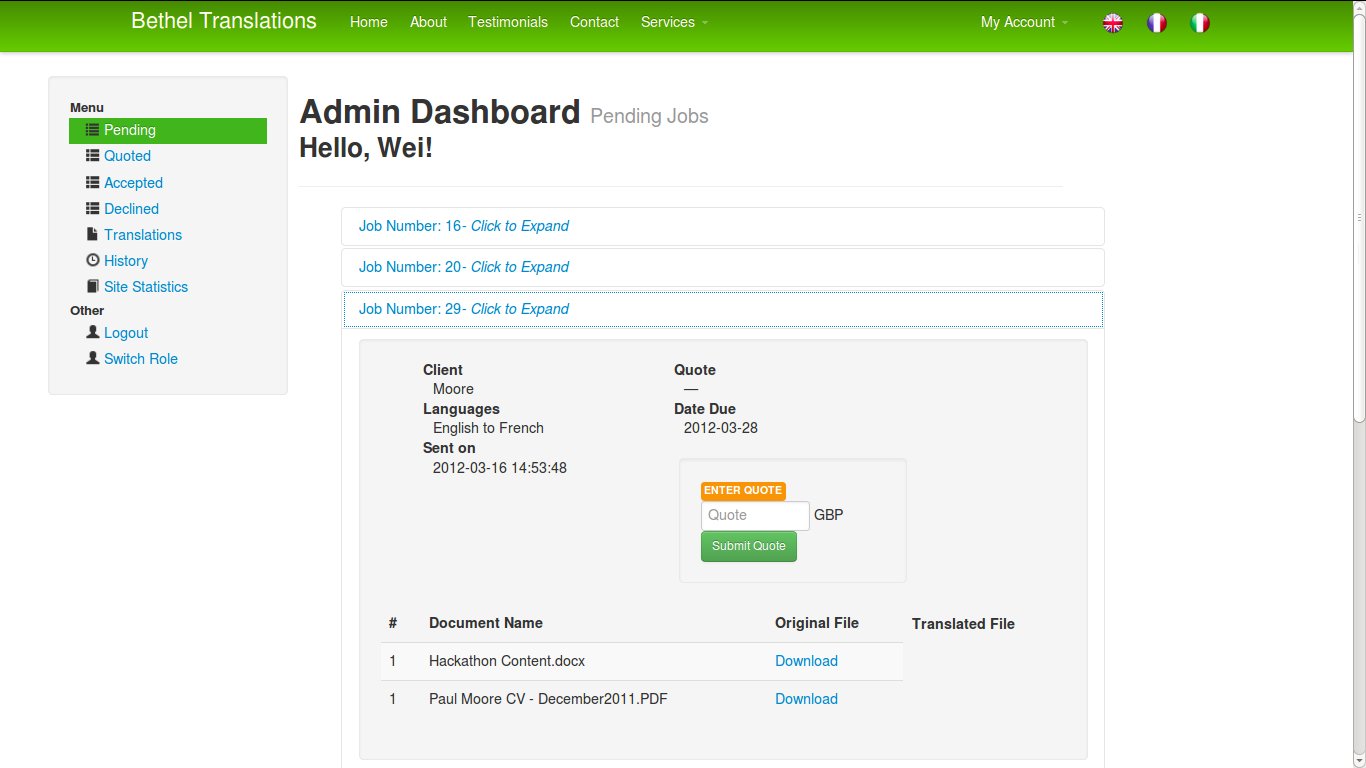
\includegraphics[width=0.8\linewidth]{images/adminDashPending}
\vspace{-30pt}
\end{figure}

\begin{itemize}
\item \textbf{Description}

This page lists all pending/quoted jobs to the translator. Information of each job will be shown in separate boxes. 
The translator can download the documents for a job and set the quote for the job here.

\item \textbf{Navigation}

The translator can get access to this page through the text link
`Pending'/`Quoted' on the side menu bar in the admin Dashboard.

\item \textbf{Main Elements}
\begin{itemize}
\item `Side Menu Bar'\\
Type: Text links\\
Content: Links to different sections of the dashboard. And the link to logout. \\
Behaviour: The user is directed to the destination of a particular link. \\

\item `Job Information'\\
Type: Text\\
Content: Information of the job including client name, source and desired languages for translation, submit date, due date, and a quote \\
Behaviour: If the job is quoted, a quote will be shown, or otherwise a dash line. \\

\item `Set/Update Quote'\\
Type: Field\\
Content: a field to input the quote and a button to confirm \\
Behaviour: A job will be moved from the pending list to the quoted list if the translator submit the quote for that job in `Pending'. The quote of the job will be updated after the translator click on `Update Quote' in `Quoted'. An email will be sent to the customer stating the the job has been updated.\\

\item `Download'\\
Type: Text link\\
Content: a download
ad link for a document in the job\\
Behaviour: -\\
\end{itemize}
\end{itemize}

\textbf{Admin Dashboard - Accepted/Declined Jobs}
\begin{figure}[H]
\centering
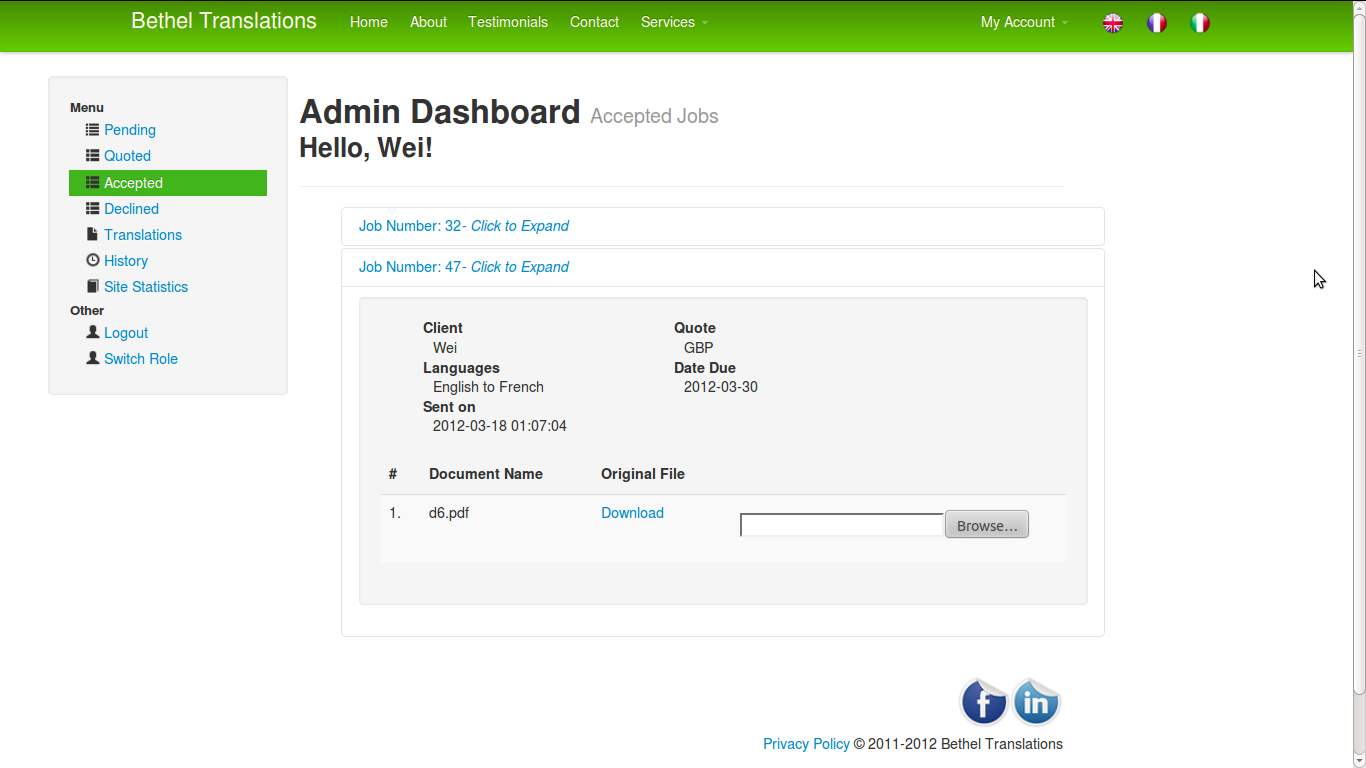
\includegraphics[width=0.8\linewidth]{images/adminDashAccepted}
\vspace{-30pt}
\end{figure}

\begin{itemize}
\item \textbf{Description}

This page lists all accepted/declined jobs to the translator. Information of each job will be shown in separate boxes. 
The translator can download the documents for a job and upload the translated documents for an accepted job here.

\item \textbf{Navigation}

The translator can get access to this page through the text link `Accepted'/`Declined' on the side menu bar in the Admin Dashboard.

\item \textbf{Main Elements}
\begin{itemize}

\item `Job Information'\\
Type: Text\\
Content: Informations of the job including client name, source and desired languages for translation, submit date, due date, and a quote \\
Behaviour: -\\

\item `Download'\\
Type: Text link\\
Content: a download link for a document in the job\\
Behaviour: -\\

\item `Upload'\\
Type: Upload Field\\
Content: A field to choose the document to be uploaded.\\
Behaviour: Only shows for accepted jobs. The accepted job will be moved to translations after the uploading is completed.\\

\end{itemize}
\end{itemize}


\textbf{Admin Dashboard - Site Statistics}
\begin{figure}[H]
\centering
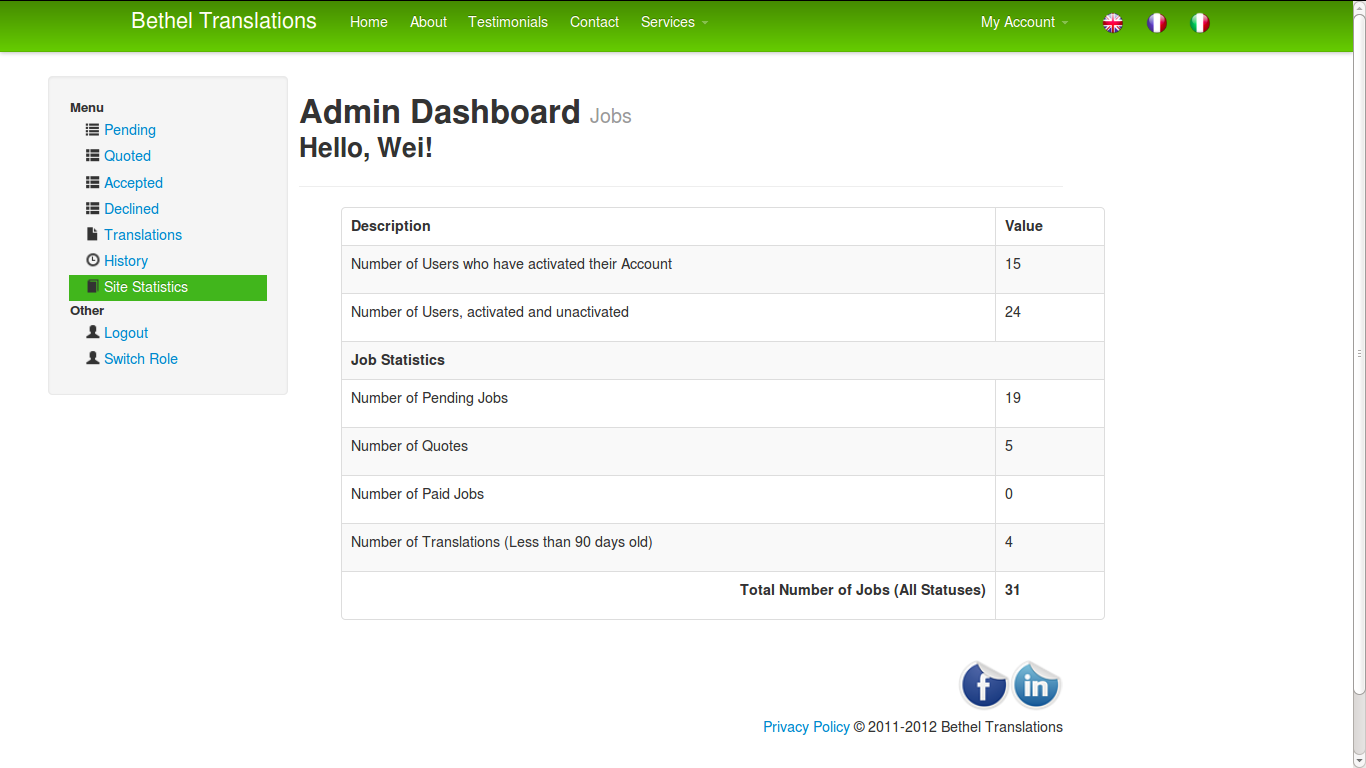
\includegraphics[width=0.8\linewidth]{images/adminDashStatistics}
\vspace{-30pt}
\end{figure}

\begin{itemize}
\item \textbf{Description}

This page lists statistic informations about the numbers of users and jobs with different status in the website.\\

\item \textbf{Navigation}

The translator can get access to this page through the text link `Site Statistics' on the side menu bar in the Admin Dashboard.

\item \textbf{Main Elements}
\begin{itemize}

\item `Statistic Information'\\
Type: Text\\
Content: Text fields showing informations about the numbers of users and jobs with different status in the website.\\
Behaviour: - \\

\end{itemize}
\end{itemize}

\textbf{Client Dashboard - Overview}
\begin{figure}[H]
\centering
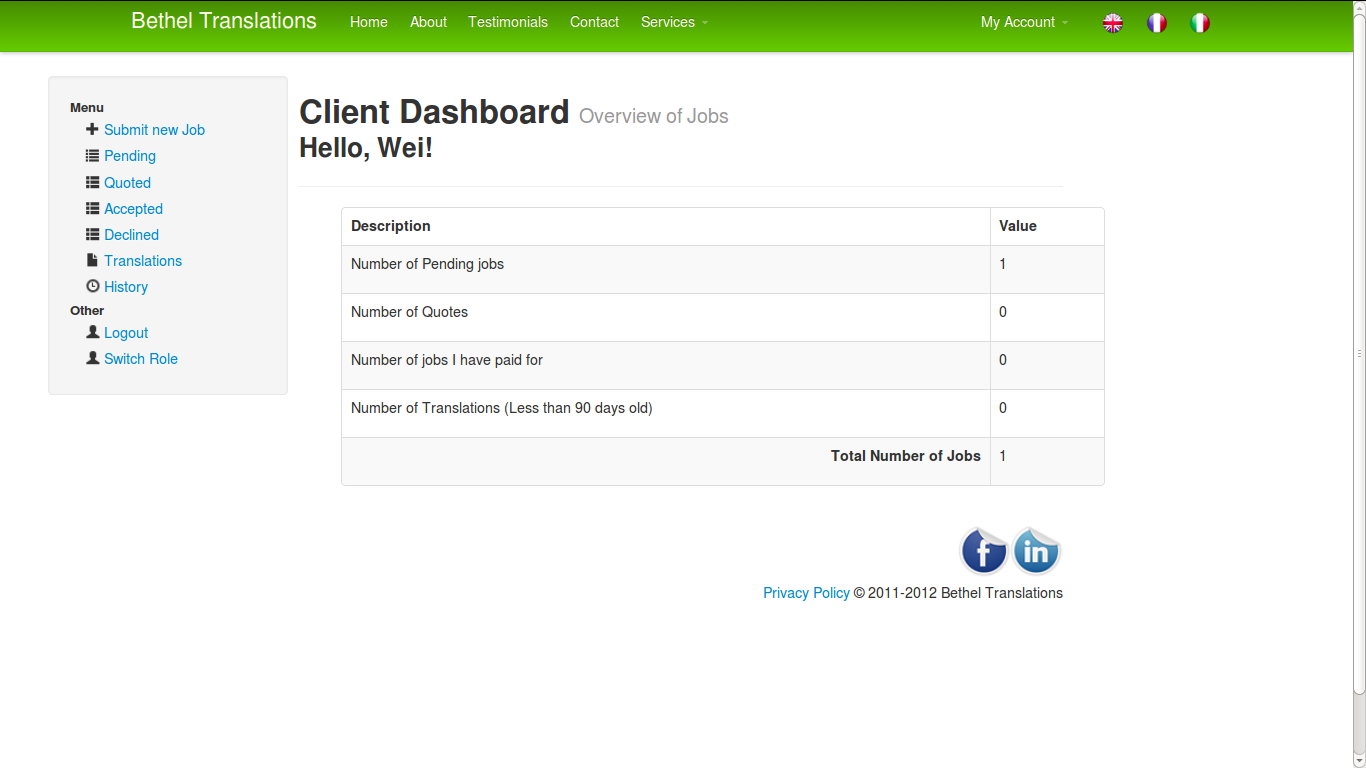
\includegraphics[width=0.8\linewidth]{images/clientDashOverview}
\vspace{-30pt}
\end{figure}

\begin{itemize}
\item \textbf{Description}

This page lists statistic informations about jobs with different status for the customer.\\

\item \textbf{Navigation}

This is the landing page when a customer come to his dashboard through the `Dashboard' link on the main menu bar.

\item \textbf{Main Elements}
\begin{itemize}

\item `Statistic Information'\\
Type: Text\\
Content: Text fields showing informations about jobs with different status for the customer.\\
Behaviour: - \\

\end{itemize}
\end{itemize}

\textbf{Client Dashboard - Submit New Job}
\begin{figure}[H]
\centering
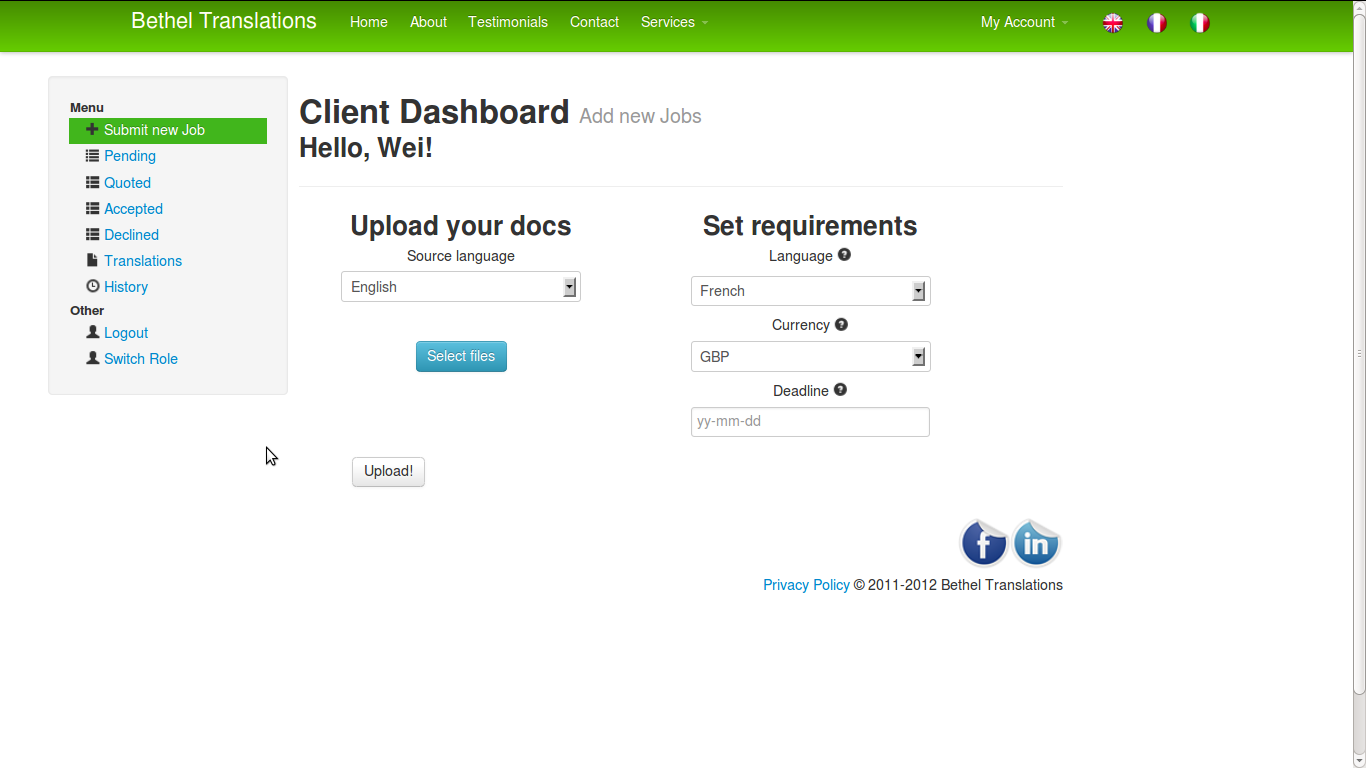
\includegraphics[width=0.8\linewidth]{images/clientDashNewJob}
\vspace{-30pt}
\end{figure}

\begin{itemize}
\item \textbf{Description}

This page is used to submit a new job by customers of the website. Except from first time customers (who will use the registration process on welcome page), 
they will be asked to come here in order to submit a new job.

\item \textbf{Navigation}

The customer can get access to this page through the text link `Submit New Job' on the side menu bar in the Client Dashboard.

\item \textbf{Main Elements}
\begin{itemize}

\item `Set requirements'\\
Type: Fields\\
Content: Fields to select requirements for `Source language', (desired) `Language', `Currency', and `Deadline' \\
Behaviour: - \\

\item `Upload'\\
Type: Button\\
Content: A  button to select files to be uploaded and a button to upload and submit a new job.\\
Behaviour: A new job will be submitted after all the requirements are set and all files are successfully uploaded.\\

\end{itemize}
\end{itemize}


\textbf{Client Dashboard - Quoted Jobs}
\begin{figure}[H]
\centering
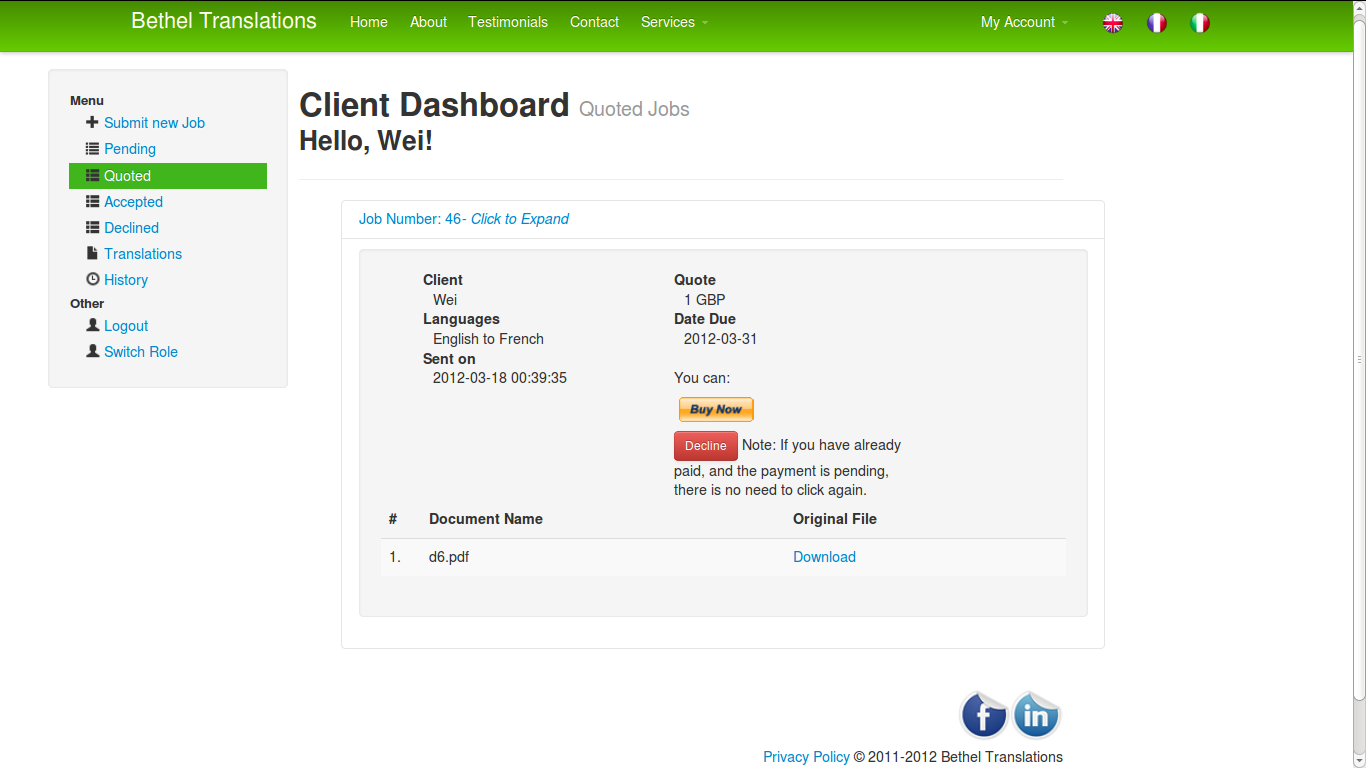
\includegraphics[width=0.8\linewidth]{images/clientDashQuoted}
\vspace{-30pt}
\end{figure}

\begin{itemize}
\item \textbf{Description}

This page lists all quoted jobs to the customer. Information of each job will be shown in separate boxes. 
The customer can accept or declined the quote here. The customer will be required to pay in order to accept a job.

\item \textbf{Navigation}

The customer can get access to this page through the text link `Quoted' on the side menu bar in the Client Dashboard.

\item \textbf{Main Elements}
\begin{itemize}

\item `Job Information'\\
Type: Text\\
Content: Informations of the job including client name, source and desired languages for translation, submit date, due date, and a quote \\
Behaviour: If the job is quoted, a quote will be shown, or otherwise a dash line. \\

\item `Accept Quote'\\
Type: Button\\
Content: -\\
Behaviour: The customer will be redirected to PayPal's secure payment system after click on it. Once he paid the job will be moved to `Accepted' section, as well as in the Admin Dashboard.\\

\item `Declined Quote'\\
Type: Button\\
Content: -\\
Behaviour: Once the customer confirm to decline the job will be moved to `Declined' section, as well as in the Admin Dashboard.\\

\item `Download'\\
Type: Text link\\
Content: a download link for a document in the job\\
Behaviour: -\\

\end{itemize}
\end{itemize}


\textbf{Client Dashboard - Translations}
\begin{figure}[H]
\centering
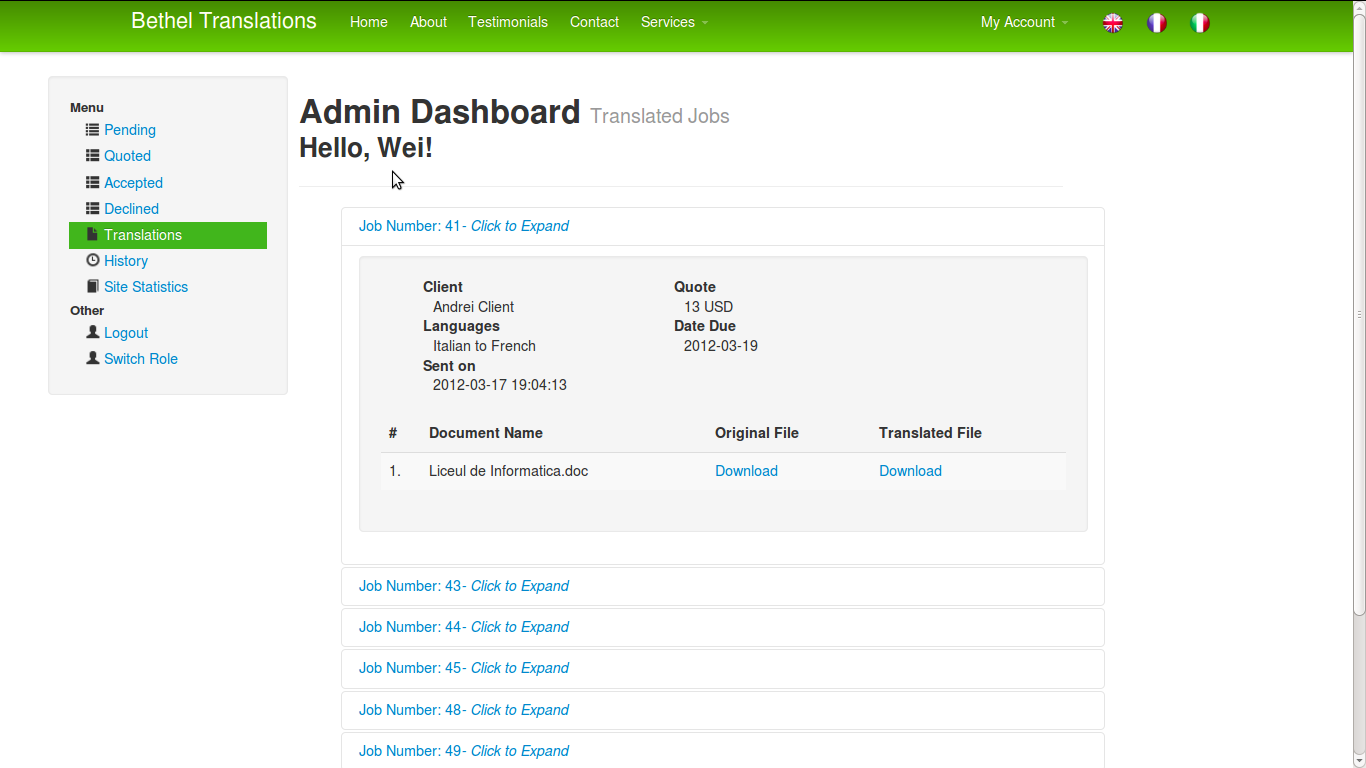
\includegraphics[width=0.8\linewidth]{images/clientDashTranslations}
\vspace{-30pt}
\end{figure}

\begin{itemize}
\item \textbf{Description}

The translated jobs will be shown here for the customer to download the documents.

\item \textbf{Navigation}

The customer can get access to this page through the text link `Translations' on the side menu bar in the Client Dashboard.

\item \textbf{Main Elements}
\begin{itemize}

\item `Download'\\
Type: Text link\\
Content: Download links for the original documents and the translated documents in a job\\
Behaviour: -\\

\end{itemize}
\end{itemize}




\section{Database Schema} \label{sect:db-sch} Having mapped the Entities
involved with Bethel Translation -  were able to integrate them in to the
database using SQL create table statements. Storing this as a script on the
development server we used allowed us to simply run it when we moved the
website to the production server and have the tables ready to use.  This
enforces a highly recommended software engineering process in that you should
always reuse code wherever possible \footnote{Software Engineering by I
Sommerville - pg 425}. Not only that, we have a script that is essentially
\textit{portable} - so it could in theory be executed on any web server and
create the tables required for Bethel Translations to function. The process of
moving the website from testing to production is described in more detail in
chapter \ref{chap:depl}  \\
\\
\small{
\textbf{Customer}\\
\\
DROP TABLE IF EXISTS `customer`;\\
CREATE TABLE IF NOT EXISTS `customer` (\\
  `customerID` int(11) NOT NULL,\\
  `fullName` text NOT NULL,\\
  PRIMARY KEY  (`customerID`)\\
) ENGINE=InnoDB DEFAULT CHARSET=latin1;\\
\\
\textbf{Document}
\\
DROP TABLE IF EXISTS `document`; \\
CREATE TABLE IF NOT EXISTS `document` ( \\
  `documentID` int(11) NOT NULL auto\_increment, \\
  `filePath` varchar(256) NOT NULL, \\
  PRIMARY KEY  (`documentID`) \\
) ENGINE=InnoDB  DEFAULT CHARSET=latin1 AUTO\_INCREMENT=11 ;\\
\\
\textbf{Job}
\\
DROP TABLE IF EXISTS `job`;\\
CREATE TABLE IF NOT EXISTS `job` (\\
  `jobID` int(11) NOT NULL auto\_increment,\\
  `customerID` int(11) NOT NULL,\\
  `status` enum('QuoteReq','QuoteSent','QuoteAccept','QuoteDeclined','Paid','Translated','Complete') collate utf8\_bin NOT NULL,\\
  `quote` int(10) default NULL,\\
  `dateRequested` timestamp NOT NULL default CURRENT\_TIMESTAMP,\\
  `dateDue` date NOT NULL,\\
  `fromLanguage` enum('english','italian') collate utf8\_bin NOT NULL,\\
  `toLanguage` enum('french') collate utf8\_bin NOT NULL,\\
  `currency` enum('gbp','eur') collate utf8\_bin NOT NULL,\\
  PRIMARY KEY  (`jobID`),\\
  KEY `customerID` (`customerID`)\\
) ENGINE=InnoDB  DEFAULT CHARSET=utf8 COLLATE=utf8\_bin AUTO\_INCREMENT=934247 ;\\
\\
\textbf{Translation}
\\
DROP TABLE IF EXISTS `translation`;\\
CREATE TABLE IF NOT EXISTS `translation` (\\
  `translationID` int(11) NOT NULL auto\_increment,\\
  `jobID` int(11) NOT NULL,\\
  `name` varchar(256) collate utf8\_bin NOT NULL,\\
  `origDoc` int(11) NOT NULL,\\
  `translatedDoc` int(11) default NULL,\\
  PRIMARY KEY  (`translationID`),\\
  KEY `origDoc` (`origDoc`),\\
  KEY `translatedDoc` (`translatedDoc`)\\
) ENGINE=InnoDB  DEFAULT CHARSET=utf8 COLLATE=utf8\_bin AUTO\_INCREMENT=5 ;\\
\\
}

%==============================================================================
\chapter{Deployment}
\label{chap:depl}
The deployment of a system involves configuring the software to operate in an operational 
environment. It involves different degrees of complexity regarding the configuration
changes that need to be made, depending on the project itself. This chapter describes 
the process followed by the team as we transported the website from one server to another: 
from a testing server used in development, to a professional web hosting company
that the translator would be responsible for managing after the project deadline.\newline
Ian Sommerville \footnote{Software Engineering, pg 385} describes that software developers 
should ``provide built-in support for deployment that will reduce the probability that system 
administrators will make mistakes when configuring the software''. Since ours is a 
website developed within a web application framework, it is relatively easy to make the
changes to accommodate this process. As the project neared the end of development stages, such
that most functional requirements of the system had been realised, more consideration was given
to non-functional requirements. It was intuitive for us that the changes be categorised 
into sections that generally match the non-functional requirements of the system.
\section{Findability}
Although the translator would already have clients lined up to use the website for translation 
services, it was still a requirement of the system to make it findable on the Internet. The Internet
is the greatest platform for advertising new companies, and the website we have developed is no different.
It is intuitive then to consider how potential customers might try and locate the service if they require it.
Undoubtedly, the majority of users would perform a search of ``document translation'' using their favourite
search engine. The challenge for us, therefore, is the increase the visibility of Bethel Translations on
these search engines. The terminology concerned is ``page ranking''. That is, the higher a page is located
in the results of a search engine query, the more likely a user is likely to click through to it. \newline
The process of increasing the visibility on search engines is known as SEO (Search Engine Optimisation). We 
looked at methods of improving this aspect of the website.  The key principle to successful SEO is using
meta-tags to increase findability via a search engine. A meta-tag is extra information contained within the HTML
that is easily readable by search engines when users enter a search query. For example, we included meta tags
such as:
\begin{lstlisting}
<meta name="description" content="Translation from English to French">
\end{lstlisting}
With these meta-tags in place, it helps search engines match pages to queries such that if a user entered ``english to
french translation'', it should increase the page ranking of that relevant page for BethelTranslations. Including
meta-tags to improve SEO is not as magical as it may seem though. The best way of increasing page visibility on 
search results is simply - time. We believe that the system we have created has provided the translator with a means
of creating a viable online business, partly due to our simple aesthetic of user interface, and partly due to our
research discussed in the \ref{sec:reliab} section later. Therefore, over time, the website can and should become
more popular.
\section{Security}
As software engineers we would be naive to believe that we should not concern ourselves with the
security of the website we had developed. A result of increasing the number of users to the site
means there is a greater security risk. The main concern with a site like this one is spam bots.
Spam bots deliberately try to misuse the site to gain access to customer information, flood the 
translator with phishing emails and various other malicious requests.\newline
We identified two areas of the site that could potentially be targeted by spam bots: the contact
page, and the main document submission/registration page. Initially it was considered to prevent 
spam bots from abusing these forms by implementing captchas. A captcha is an interactive form that
presents some audio-visual information that only a human can interpret and provide the system with 
the confirmation that they are using it for genuine purposes. However, there existed a simple 
solution than this one: hidden form validation. It is a simpler and far less intrusive approach that
exploits the way spam bots use forms. It also meant we didn't have to concern ourselves with 
cross browser compatibility which can be a headache with including captchas in a website. In our HTML
for the aforementioned pages, we included two input forms amongst all the other genuine ones. The 
difference with these two forms is that they include the ``hidden'' tag. The general form of these is:
\begin{lstlisting} 
<input type="hidden" value="">
\end{lstlisting}
There is a simple beauty to this method of anti-spam bot detection: the genuine users are never aware of the
existence of it. However, spam bots will typically fill in every html form they can find in order
to achieve their goal. Some simple JavaScript check that looked at the value field in the code snippet above
was then enforced. If the hidden forms were filled in, the page wouldn't allow the registration or contact 
query to go through. 
\section{Marketability}
The challenge of encouraging potential customers to try the website does not end with them finding it, although 
that is a major part of the problem. Once they have navigated their way to the website, it is extremely important 
that we entice them somehow into committing to the process of signing up and submitting documents for translation.
We believed we had accomplished this somewhat already via our simple, aesthetically pleasing interface design.
At the end of the development phase, however, the translator had sent us some plain text for some of the static 
pages contained in the website. These included vital information on things like the other services she offered
and information about her experience as a translator. The team modified this plain information into styled pages
that were consistent with the rest of the website. Phrases such as ``free full quote'' were emboldened. We 
aimed to emphasise some attractive features of the service as subtly as possible. These changes may seem 
trivial on first impressions, but the study at \small{\textit{\url{http://sixrevisions.com/usabilityaccessibility/10-
usability-tips-based-on-research-studies/}}} suggests that giving a little thought to the potential customers
and how they interact with the website can benefit it hugely.
\section{Reliability}
\label{sec:reliab}
Another extremely important aspect of the deployed system would be to ensure it was reliable. In the 
Professional Software Development lectures, we are taught that {software maintenance} accounts for
\textbf{over 90\%} of the workload in software engineering projects. Since we would not be responsible for 
maintaining the system after deployment, and given the inability of the translator to do this 
herself, we hand picked a rigorous server for the website to be hosted on. This decision was reached after
careful evaluation of available hosting plans. The hosting company we decided on is located at 
\small{\textit{www.krystal.co.uk}}. In brief, it offers afforable, competitive plans and is situated in a 
``bunker data-centre''. We were able to find an excellent plan for the translator that involved,a among other
 great perks, 50GB of storage and email accounts.
We realised the latter to be important to her as she was intent on sending emails under a company
name, not her own personal account. The hosting company is well reputed and states that it has a system in place
to take frequent backups of data, excellent physical security and round the clock customer support. We were
more than happy to recommend this company for Joelle to host her website on purely because of the reliable
service on offer and, thankfully, the agreement was mutual.
\section{Configuration}
The final section of this chapter provides a summary of the steps followed to port the website code base over
from development to production.

The actual deployment of the website consisted of a number of important steps:
\begin{itemize}
	\item \textbf{Setting up the database} - the database schema was kept under
		version
		control as an SQL file, which was used in an installation script that
		would create the tables.
	\item \textbf{Uploading} and \textbf{configuring} the application on the
		server - this was
		very straightforward, since we only had to upload the files from our
		testing server to the Bethel Translations one. Codeigniter natively 
		supports configuration files for its modules, but only one of them
		was actually related to the domain name on which the application was
		installed and needed to be changed.
\end{itemize}

%==============================================================================
\chapter{Evaluation}
\label{chap:eval}
First feedback with Karen including wire-frames etc - Jan 25\\
Second feedback session with Karen incl more complete website design - Feb 9th\\
\\
Successful evaluation of a software project is paramount. Without it,
developers are left to their own volition, assuming all the decisions they've
made are the correct ones. Developers cannot presuppose every vector of user
behaviour, neither can they recognise every error in the source code. Carefully
observing and recording user interactions with the system is a valuable tool
in pin-pointing errors of judgement and failures in implementation.\\
\\
In this project, a transaction involves multiple staged exchanges
between our client and the customers. Feedback was crucial in order to confirm
that our decisions made at the design stage stood up to the challenges of
everyday use.

\section{User Testing}
\label{sect:testing}
Although we performed regular evaluations of the system throughout the development
period, it was necessary to coordinate a comprehensive evaluation strategy to
fully road test our system once it was largely feature complete and operational.
Taking place in the computing department's level 3 laboratory.  At the same time
carefully selected individuals out-with the university were invited to take
part.\\
\\
Evaluators were given instructions on how to access the website and a task sheet
to complete. Immediately following the evaluation, participants were invited to
fill out an online questionnaire, detailing any problems encountered throughout the
session and offering the ability to leave and suggestions.\\
\\
Six people in total completed the evaluation, of which five were present during the
lab session. Overall, the responses were very favourable, and we will list the
full results in appendix \ref{sect:survey-results}. Below are some highlights
from the evaluation process, with attention drawn to notable results and issues
raised.

\subsection{Interface}
The general consensus taken from the evaluation is that the vast majority were
happy with the `3-steps' design and processes involved in purchasing the translation
service. Particular credit was given to the client dashboard. Users found
interacting with and tracking their documents intuitive and the interface
responsive. The colours used, layout of the pages and the browser features employed (such as
expanding areas of the dashboard) were all appreciated by the participants.
 
\subsection{Problems}
Some issues were raised during the tests, particularly during the lab evaluation
session. Most notably, the PayPal stage was a block to the participants
completing the task's asked of them. Due to an incorrectly set API key,

\subsection{Suggestions}

\section{Client Evaluation}
\label{trans-eval}
TODO how to describe this?!

%==============================================================================
\chapter{Conclusion}
\label{chap:concl}

When we started the project in September we didn't know each other, every member had varying knowledge of
web development techniques, and we were worried about not meeting the clients requirements. This ensured that the project tested each team member’s intelligence
and desire to learn. The following section revises the main aims, summarises the achievements and
what we learned, and then suggests possible future work for the project.

%==============================================================================
\section{Aims}
\label{sect:aims}
TBC

\section{Achievements}
\label{sect:achv}
Now that we have reached the conclusion of our project there are several parts that we see as achievements.
That we have a working and complete system is a great achievement. In September we had hopes
and ambitions of what the website would do. As time progressed and as we learned our limits due to using new
programming languages, there were times when it seemed like the project may never have reached a stage where 
we could consider it complete. We are extremely glad to have a working product to be able to give to our client.

A second achievement is on a personal level for the team. We as a group did not know each other before the project.
That we have come together and worked well as a team to achieve our end goals can be seen as an achievement as we have
successfully completed the task we were given, together.

\section{Future Work}
\label{sect:fut-work}
\begin{itemize}
\item{Languages}

Since our client, the translator, did not have enough time to translate the website into languages other 
than English, for the moment we have only fully deployed the website in its English version. 
But it will easy enough to have a version in another language within the framework we are using. We have 
actually partly implemented the website in French and Italian. It will be only about listing the corresponding 
translations of the texts in the website in one place within the framework.

\item{Currencies}

As the translator requires we only let customers to pay in 3 different currencies, namely Dollers, Euros and Stirling Pounds. 
However, it is always possible to support payment using some other currencies. In the background we have integrated 
PayPal to deal with the payment and it will automatically exchange the currency for the translator. 

\item{Payment Types}

We will consider adding Bacs\footnote{\url{http://www.bacs.co.uk/}} as a payment method alongside PayPal as a possible extra feature for the future work.

\item{User Profiles}

One thing we may provide in the future work is the user profile page. That is, the translator will be able to select a particular 
user and view his profile and past business history with him. This may potentially require the registerd users of the website to 
complement more of their informations.

\end{itemize}
\section{Contributions}
\label{sec:contrib}
As is discussed in the project plan, the team had a very open and agile approach to the project.
All members of the team have worked on various parts of the project. 
We realised the dissertation was one of the most major parts of the project and it was therefore decided that
every member of the team would work on this document, irrespective of what part of the project they had worked on previously.
Individual Contributions are summarised in the paragraphs below.

Alasdair Campbell contributed to the project in the following areas, among others:
\begin{itemize}
\item{Implementation of File Uploads}
\item{Implementation of Database}
\item{Implementation of Language Functionality}
\item{Writing of Evaluation Section of Dissertation}
\item{}
\item{}
\end{itemize}
Stephen Hayton contributed to the project in the following areas, among others:
\begin{itemize}
\item{Main communicator with translator}
\item{Transforming translator feedback to website refinements}
\item{Writing of Deployment and Introductions of Dissertation}
\item{Maintaining the style of website through CSS and JS updates}
\item{Fixed issues mainly with erroneous inputs to site}
\item{Some UI fixes for cross platform compatibility}
\end{itemize}
Andrei Mustata contributed to the project in the following areas, among others:
\begin{itemize}
\item{Implementation of Registration, Documents Transitions, Authentication.}
\item{Advocated use of Twitter Bootstrap.}
\item{Written Implementation of Dissertation.}
\item{Made the Prototype and Wire-frames.}
\item{Carried out daily testing of new features.}
\item{Carried out final deployment moving from test server to Bethel Translations server.}
\end{itemize}
Paul Moore contributed to the project in the following areas, among others:
\begin{itemize}
\item{Writing of Project Plan, Introduction, Development Environment and Conclusion areas of Dissertation}
\item{Maintaining the style of website through CSS and JS updates}
\item{Implementation of Contact page and Navbar Login}
\item{Implementation of Site Statistics}
\item{Carrying out the Evaluations}
\item{Organisation of Project Demonstration and Final Presentation}
\end{itemize}
Wei Zhang contributed to the project in the following areas, among others:
\begin{itemize}
\item{Led the progress presentation}
\item{Taking minutes of weekly meetings and making sound records for important meetings}
\item{Research and the implementation of the PayPal feature (with Andrei)}
\item{Researched other websites and brought up the basic idea of the 3-steps process on the main page}
\item{Writing Design and User Process section of Dissertation}
\end{itemize}	

%==============================================================================


%==============================================================================
\bibliographystyle{plain}
\bibliography{example}
\appendix
\chapter{Glossary of Terms}
\label{chap:gloss}

\begin{itemize}
\small{
\item{\textbf{API} - Application Programming Interface. The source-code level specification for interactions between computer systems.}
\item{\textbf{LAMP} - LAMP, (Linux, Apache, MySQL and PHP), is an acronym for a solution stack of free, open source software}
\item{\textbf{Open source} - Computer software for which the code is freely available }
\item{\textbf{Programming language} - A programming language is an artificial language designed to express computations that can be performed by a computer.}
\item{\textbf{Requirement gathering} - Determining the needs of a client through any form of communication.}
\item{\textbf{Software project} - Using the surrounding context, a software project aims to create application(s) using programming language(s) by adhering to project management principles.}
\item{\textbf{Web application framework} - A software framework that is designed to support the development of dynamic websites }
\item{\textbf{Web scripting language (\textit{PHP, JavaScript})} - A scripting language is a programming language that allows control of one or more applications.}
\item{\textbf{Website development} - The process of constructing and maintaining a website.}
}
\end{itemize}
%==============================================================================
\chapter{Bibliography}
\label{chap:bibl}
Any externally owned items referenced throughout this document have been sourced
at the web addresses/textbooks below:
\begin{itemize}
\small{
\item Example ref here.
}
\end{itemize}
%==============================================================================
\chapter{Project Plan}
\label{chap:proj-plan}
\section{Introduction}
\label{sect:pp-intro}
\subsection{Identification}
This is the Project Plan for the Website for a Translator project by Team O.

\subsection{Purpose and Description of Document}
This project plan sets out all the details of the project and defines all the
necessary work that must be undertaken to 
fulfil the project. It will be used as a reference guide by the team to make
sure that the project stays on time, and that all tasks 
that need to be undertaken happen according to schedule, in the correct order to achieve completeness.

\section{Resources, Budgets, Schedules and Organisation}
\label{sect:rbso}
\subsection{Work Breakdown Structure} 

\begin{center}
    \begin{tabular}{ | l | p{12cm} |}
    \hline	
    Task 1 & Group Organisation \\ \hline
    Description & A document will be written following discussion with the team as to how the
	team will work and what our methods of communication, storage and backup will be. \\ \hline   
    Outcomes & The team will have clearly defined roles and each member will be able to contact all members of the team in defined ways. \\ \hline
    Deliverables & Team Organisation Document. \\ \hline
    Risks & Team members may be disappointed with role or may not agree on structure. \\ 
    \hline
    \end{tabular}
\end{center}

\begin{center}
    \begin{tabular}{ | l | p{12cm} |}
    \hline	
    Task 2 & Scheduling and Planning Meeting \\ \hline
    Description & A meeting will be held with the team to discuss our planning methods and scheduling of resources. \\ \hline   
    Outcomes & The basis of a project plan. \\ \hline
    Deliverables & None \\ \hline
    Risks & Certain events might be scheduled when a team member is unavailable. \\ 
    \hline
    \end{tabular}
\end{center}

\begin{center}
    \begin{tabular}{ | l | p{12cm} |}
    \hline	
    Task 3 & Project Plan \\ \hline
    Description & A Project Plan will be written which the team can use to keep track of the state of the project. This will allow sufficient division of human resources to different aspects of the project. \\ \hline   
    Outcomes & Project Plan \\ \hline
    Deliverables & Project Plan \\ \hline
    Risks & None \\ 
    \hline
    \end{tabular}
\end{center}

\begin{center}
    \begin{tabular}{ | l | p{12cm} |}
    \hline	
    Task 4 & Research \\ \hline
    Description & As a pre-requisite to requirements gathering we must research the current trends in web-development and research what works and doesn't work in a user friendly website. \\ \hline   
    Outcomes & The team will have an understanding of what current design practices are in use and what we must achieve to be competitive in the market. \\ \hline
    Deliverables & None \\ \hline
    Risks & None \\ 
    \hline
    \end{tabular}
\end{center}

\begin{center}
    \begin{tabular}{ | l | p{12cm} |}
    \hline	
    Task 5 & Requirements Gathering Interview \\ \hline
    Description & An interview plan will be written, consisting
          of the objectives of the interview, questions to be asked and
          identification of the roles in the interview. During this task our initial research will be brought together, including the discussion of the use cases involved in the task. It will then be
          reviewed, edited and approved before going to interview the translator. \\ \hline   
    Outcomes & The team will have a firm understanding of what the translator wants the website to achieve and will be able to continue the process of development in a now fully informed manner. \\ \hline
    Deliverables & None \\ \hline
    Risks & If we do not ask the right questions we may not gather enough information about the system and will have a flawed understanding of what we must achieve. \\ 
    \hline
    \end{tabular}
\end{center}

\begin{center}
    \begin{tabular}{ | l | p{12cm} |}
    \hline	
    Task 6 & Specification and Requirements Document \\ \hline
    Description & Following analysis of the interview write-up, create a requirements document from the specification as set out by the translator. \\ \hline   
    Outcomes & Formalised requirements document. \\ \hline
    Deliverables & Requirements Document \\ \hline
    Risks & Client may change their mind or team may have received inaccurate requirements. \\ 
    \hline
    \end{tabular}
\end{center}

\begin{center}
    \begin{tabular}{ | l | p{12cm} |}
    \hline	
    Task 7 & Prototype \\ \hline
    Description & Creation of a paper prototype to show to the translator to confirm that the requirements gathering process was correct and that we have a deep understanding of what the translator wants from the system. \\ \hline   
    Outcomes & Confirmation of correct requirements or list of amendments needed to match requirements. \\ \hline
    Deliverables & Paper Prototype \\ \hline
    Risks & The prototype may consume too much time if the plan is not followed, therefore causing delay in meeting deadlines. \\ 
    \hline
    \end{tabular}
\end{center}

\begin{center}
    \begin{tabular}{ | l | p{12cm} |}
    \hline	
    Task 8 & Revision of Requirements \\ \hline
    Description & From the Paper Prototype task the team will have received a list of things that need changed to match the translators requirements. These will be incorporated into the requirements document. \\ \hline   
    Outcomes & Requirements updated to what the translator wants. Team now has correct understanding \\ \hline
    Deliverables & Revised Requirements Document \\ \hline
    Risks & Translator may see this as an opportunity to add further functionality to the specification. \\ 
    \hline
    \end{tabular}
\end{center}

\begin{center}
    \begin{tabular}{ | l | p{12cm} |}
    \hline	
    Task 9 & Static Page Implementation \\ \hline
    Description & Implementation of the basic site, with only static pages and template. \\ \hline   
    Outcomes & Basic Website live on site \\ \hline
    Deliverables & None \\ \hline
    Risks & The implementation may consume too much time if the plan is not followed, therefore causing delay in meeting deadlines. \\ 
    \hline
    \end{tabular}
\end{center}

\begin{center}
    \begin{tabular}{ | l | p{12cm} |}
    \hline	
    Task 10 & Dynamic Page Implementation \\ \hline
    Description & Complete implementation, including all document uploads, client and admin dashboards, PayPal implementation and Contact forms. \\ \hline   
    Outcomes & Full version of website available online \\ \hline
    Deliverables & None \\ \hline
    Risks & The implementation may consume too much time if the plan is not followed, therefore causing delay in meeting deadlines. \\ 
    \hline
    \end{tabular}
\end{center}

\begin{center}
    \begin{tabular}{ | l | p{12cm} |}
    \hline	
    Task 11 & Testing \\ \hline
    Description & Members of the team with less involvement in the development of the website will now fully test the site to check that the implemented functionality matches the requirements stated. \\ \hline   
    Outcomes & The team will have a list of known faults that need to be fixed and an understanding of what works well and what does not. \\ \hline
    Deliverables & None \\ \hline
    Risks & Although some members of the team will have had less involvement in the development, everyone has some understanding. The team have a biased view of what should and should not happen. This could lead to testing that is not 100 percent effective. \\ 
    \hline
    \end{tabular}
\end{center}

\begin{center}
    \begin{tabular}{ | l | p{12cm} |}
    \hline	
    Task 12 & Translator Evaluation \\ \hline
    Description & The translator will be given a list of tasks and a questionnaire to complete in order to fully evaluate the site we have developed. \\ \hline   
    Outcomes & The team will learn what the client likes or dislikes about the website. \\ \hline
    Deliverables & Evaluation Report \\ \hline
    Risks & Ethics Approval \\ 
    \hline
    \end{tabular}
\end{center}

\begin{center}
    \begin{tabular}{ | l | p{12cm} |}
    \hline	
    Task 13 & Customer Evaluation \\ \hline
    Description & Both potential and fake customers will be given a list of tasks and a questionnaire to complete in order to fully evaluate the site we have developed. \\ \hline   
    Outcomes & The team will learn of what works and does not work about the site, getting feedback on why certain parts did or did not work. \\ \hline
    Deliverables & Evaluation Report \\ \hline
    Risks & Ethics Approval \\ 
    \hline
    \end{tabular}
\end{center}

\begin{center}
    \begin{tabular}{ | l | p{12cm} |}
    \hline	
    Task 14 & Dissertation \\ \hline
    Description & A full report of the project, including: design; implementation and evaluation conclusions. This is to allow our supervisor and reader to learn about what we did, how we did it, and what did or did not work in our project. \\ \hline   
    Outcomes & Completed Dissertation \\ \hline
    Deliverables & Dissertation \\ \hline
    Risks & Dissertation may not be to acceptable standard, may be too long or too short or contain irrelevant material. \\ 
    \hline
    \end{tabular}
\end{center}

\begin{center}
    \begin{tabular}{ | l | p{12cm} |}
    \hline	
    Task 15 & Project Presentation \\ \hline
    Description & We will present a detailed description of how we went about taking this project from an idea to a completed piece of software. This will include a demonstration of the completed software. \\ \hline   
    Outcomes & Project Presentation \\ \hline
    Deliverables & None \\ \hline
    Risks & Not all team members are keen public speakers - this may detract from the quality of the presentation. \\ 
    \hline
    \end{tabular}
\end{center}

\subsection{Resource Estimation and Allocation to WBS}
We have five team members available to us. It is expected that each member will spend around 5 to 8 hours a week on project giving us a sum total of 25 to 40 man hours spent on the project each week.

Other resources, as given to us by the Computing Science department, include a
computer laboratory where we can undertake the necessary work to complete the
project and access to a meeting room in Level 7 where we can have our
individual team meetings.

Allocating these resources will be done on an ad-hoc basis in order to meet the deadlines and deal with the tasks according to the project schedule.
One person will take overall responsibility, but everyone has an equal part in completing the tasks in the project plan.

\subsection{Schedules}

\begin{figure}
\begin{center}
\label{fig:gantttasks}
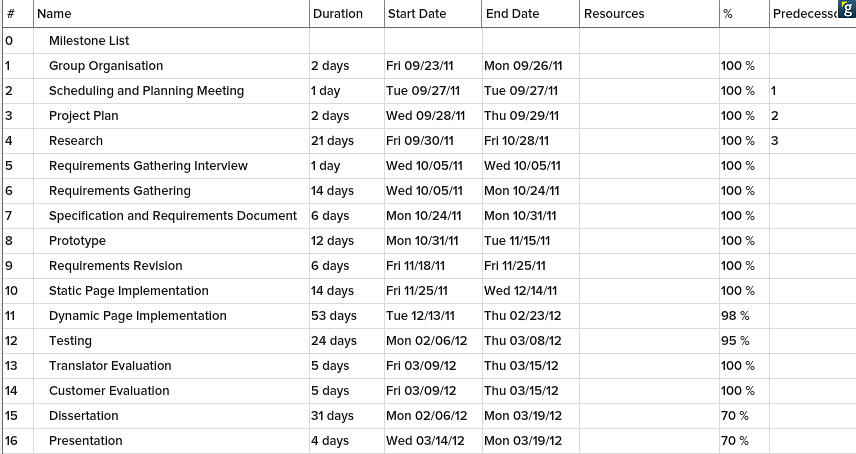
\includegraphics[scale=0.5, angle=90]{images/tasks}
\caption{\small{Task Schedule - matching Gantt Chart Tasks}}
\end{center}
\end{figure}

\begin{figure}
\begin{center}
\label{fig:ganttchart}
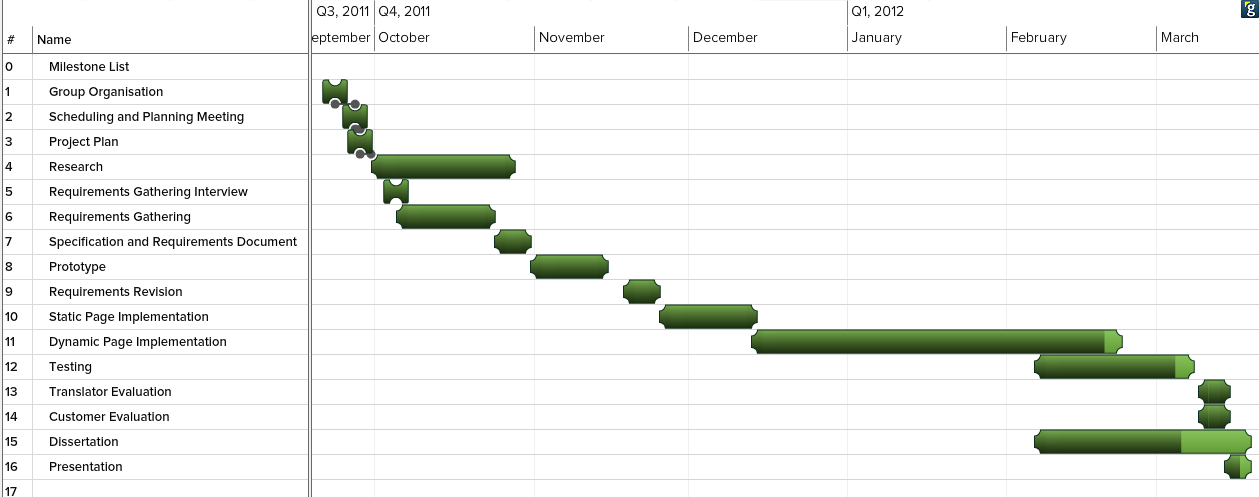
\includegraphics[scale=0.5, angle=90]{gantt}
\caption{\small{Gantt Chart}}
\end{center}
\end{figure}

\newpage
\section{Organisation}
\label{sect:org}
At the beginning of the project the team were uncertain as to who was most skilled in specific areas so it was decided that everyone would be involved in all stages of the project, to varying levels. As the project progresses it will become clear who is a strong leader in specific areas and those members will then be able to lead the way for that part of the project.

To make sure that, should a situation arise, there is always someone responsible for all tasks, we have assigned basic roles to everyone as follows

\begin{itemize}
\item{\textbf{Project Manager - Stephen Hayton} - First point of communication between the group and the customer. Chairs meetings and maintains the project’s schedule.}
\item{\textbf{Toolsmith - Andrei Mustata} - Researches and trains the group in any new software required to fulfil the task.}
\item{\textbf{Librarian -Alasdair Campbell} - Maintains the team’s documentation including minutes of meetings, the project schedule, trac.}
\item{\textbf{Quality Assurer - Wei Zhang} - Manages testing, assuring compliance with any requirement specification documents.}
\item{\textbf{Configuration Manager - Paul Moore} - Organises modifications to the software project, maintains the version control system and enforces agreed coding standards.}
\end{itemize}

There is enough overlap of the roles to overcome the situation of a member being unable to attend
meetings due to illness.

\section{Information Management}
\label{sect:info-man}
Our project data will be held on an SVN server with access rights given only to
members of the team. This SVN server is hosted with Google, on Google Code. This
means our project is open source. This is a requirement of using the CodeIgniter
framework without having to pay for a license. 

We also have a test server, to which we upload a second copy of everything from
the SVN. This allows us to see the website as it will look on a browser viewed
from a live web server. We have a script that we can run that will make sure
everything that is on the server is also on SVN so that we do not loose work.

\subsection{Communication} Our primary communication channel will be a mailing
list, with every message archived on a server. Only members of the group can
send messages to the team through the mailing list. Other methods of
communication that we will use are: \begin{itemize} \item \textbf{Facebook} -
Closed group page accessible by each member of the team, with ability to share
multimedia content and instant messaging.  \item \textbf{SMS/Phone} - Numbers
were exchanged which proves a useful form of communication when a team member
can't attend a meeting due to illness, for example.  \item \textbf{Google Shared
Calendar} - Every member can view and amend a group calendar set up on a GMail
account.  \item \textbf{Face to Face Meetings} - Every member will attend a
weekly (or more frequent if needed) meeting to discuss progress.  \end{itemize}

\subsection{Equipment, Materials, Facilities, and Other Resources} A wide
variety of machines were used for the tasks in the project. The dissertation and
reports were mainly written on lab machines in the Level 7 lab.  The
implementation was carried out mainly from home on team members individual
personal computers and laptops running Windows and Linux. \newline During the supervised meetings notes
were taken and distributed to the mailing list.  The backups taken of documents
were stored in various locations, such as on the university machines and at
home. This provided a reliable backup and redundancy in case of media failure in
one location. The backups of the test server were carried out in a similar
fashion in case of server failure.

\section{Assurance Plan}
\label{sect:a-plan}                                                                               
From our Professional Software Development course we have learnt that quality
assurance is a major part of software development. From mistakes made in the
past we now know that at least one member of the group should be appointed as
Quality Assurer. This will minimise the risk of submitting poorly written code,
documents or presentations and will greatly increase the standard of submitted
work. This Quality Assurer should be a member of the team who is independent of
the development team. This will allow them to report on quality issues without
being influenced by the issues arising from software development. In a small
team of five people it will be impossible to have a completely independent
member being quality assurer however having people play to their strength means
that one or two team members will be less involved with coding than others.

Quality Assurance will be carried out through all stages of the project: making
sure that we adhere to set plans and deadlines, checking the standard of code
submitted to the repository, and also spelling and grammar checking of the
deliverables and dissertations.

These reviews and inspections, when used along with software testing, will
allow us to validate our requirements and verify that our software does what we
intended it to. The document reviews will insure that we right a document that
is fitting to properly explain and describe all that we have achieved.

\section{Risk Management Plan}
\label{sect:risk-man}
Risk Management is an important part of any project. Risk Management Plans
involve anticipating risks that might affect the project and creating
contingency plans that will allow for the risk to be avoided or at least the
effect of the risk to be minimised.

\subsection{Risk Identification and Analysis} 
The identification of risks was initially handled at the Group Organisation
meeting, and then later expanded upon in the Planning meeting. Everyone
commented on potential risks personal to them and then we brainstormed as a
team to come up with risks that may externally affect the project.

For all risks discovered we must:
\begin{itemize}
\item{\textbf{Discover the root cause of the risk.}}
\item{\textbf{Categorise the risk (e.g. catastrophic/critical/marginal/negligible).}}
\item{\textbf{Minimise the risk if not remove it completely.}}
\item{\textbf{Document the risk and how it was dealt with.}}
\end{itemize}

Once the risks have been documented it is common practice to assign them a
threat level so that lower level risks can be separated out from risks that may
cause a catastrophic problem to the project.

The threat levels that will be used are as follows:
\begin{itemize}
\item{\textbf{Insignificant:} Slight inconveniences to the project.}
\item{\textbf{Tolerable:} Project is inconvenienced. There may be a potential to recover to stick to schedule.}
\item{\textbf{Serious:} Would involve significant project degradation. Would
		take considerable team effort to fix and the viability of completing the
		project would be questioned.}
\item{\textbf{Catastrophic:} Potential project abandonment due to risks that are out-with our control or to serious to recover from.}
\end{itemize}


\subsection{Monitoring}
It is important to track any risks once identified. If a risk is identified as
negligible at one stage and ignored for too long the severity of the risk may
increase because we have simply worked around it and not removed it. Issues
will be added to our issues list, functionality that is provided through Google
Code SVN. The issue will be assigned a risk factor and the list will be
reviewed by the team weekly.

\subsection{Avoidance}
As the project life-cycle develops, choices will be made as to whether or not
to change aspects of the software design to avoid risks that may be introduced
as a result. 

\subsection{Review}
Risk will be monitored through our web-based issues list. These issues and
risks will be discussed at our weekly meetings with team members giving their
view on whether an issues poses significant risk to be acted upon. If any
concerns are highlighted then the team will take action to resolve the issue.

\subsection{List of Managed Risks}

\begin{center}
    \begin{tabular}{ | p{4cm} | l | l | p{4cm} |}
    \hline
    Risk & Probability & Impact & Trigger \\ \hline
    Personnel shortfall at crucial development stages & Low & Serious & Illness, other commitments  \\ \hline
    Unrealistic schedule not adhered to & Medium & Tolerable & Improper planning of work time line \\ \hline
    Inaccurate requirements capture & Medium & Serious & Miscommunication with client \\ \hline
    Lack of technical knowledge in team (PHP, HTML, CSS, JavaScript) & Low & Catastrophic & Lack of commitment
    to other university courses or weakness in understanding \\ \hline
    Shortfall in externally performed tests & Low & Insignificant & Laziness, misguided belief that software is fully secure \\ \hline
    Team Members external commitments & Medium & Tolerable & Team member has commitments that prevent them carrying out team tasks \\ \hline
    Requirement volatility - Client demands change & Medium & Serious & Client has change of circumstances e.g. budget, time, mind-set \\ 
    \hline
    \end{tabular}
\end{center}

Other risks that have not been planned for in this section are discussed in specific areas of the main project dissertation.

\section{Configuration Management Plan}
\label{sect:conf-man}

The team will identify all items that must be managed as part of the configuration management plan.
This includes code,documents,and images that the team decide are necessary to be managed.

A baseline will be agreed upon for all files under management. This means all files will be reviewed and
agreed upon and then serve as the basis for further development. This means there is always a base line
of the last working version.

Diagram C1 outlines the process for Configuration management. 
All changes to the managed files are committed to the SVN where they are reviewed by the configuration
manager and assessed to be acceptable or unacceptable. They are then added to the baseline or labelled
as needing more work before being baselined.

\begin{figure}
\begin{center}
\label{fig:configman}
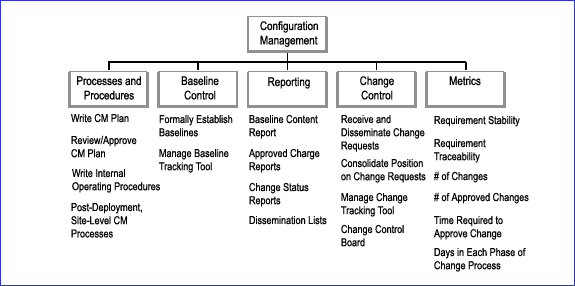
\includegraphics[scale=0.6]{config}
\caption{\small{Configuration Management Activities, source: http://www.goldtech2000.com/images/image014.gif}}
\end{center}
\end{figure}


%==============================================================================
% Specified as required subsidiary information
\chapter{Problem Definition}
\label{chap:prob-spec}
\section{Problem Title - Website for a Translator}

This project is suitable as a software engineering project. It may require participation from people
other than the student and the supervisor as part of the evaluation.

You are going to develop a system for a free-lance Translator. The system should do the following:

\begin{itemize}
\item{Advertise the translation system (attractive page)}
\item{Register new users}
\item{Allow people to upload documents and set "to" and "from" languages}
\item{Allow them to log in and see the progress of their document}
\item{When the translation has been done, the system sends them an e-mail and they can log in and fetch their translated file}
\item{Linkage with PayPal to get payment sorted}
\item{Admin page to provide an overview of exactly what work needs to be done}
\item{An e-mailed newsletter to regular clients at regular intervals}
\item{A feedback page where people provide testimonials to prospective customers}
\item{Related products which can be bought (and paid for via PayPal)}
\item{A link to Facebook}
\end{itemize}


%==============================================================================
\chapter{Evaluation Documents}
\label{chap:eval-docs}
\section{Introduction and Consent}
\label{sect:intro-cons}
\textbf{Bethel Translations – Evaluation Consent Form}\newline
This evaluation will take about 20 minutes to complete. 
You may ask as many questions as you like before the evaluation starts. The
tasks you have to carry out will be provided to you on another sheet. You are
asked to circle YES if you successfully complete a task or NO if the
opposite.\newline
When uploading files please do not upload private or assessed documents –
lecture PDFs are an example of a good document to upload. All documents will be
deleted after the evaluation and will not be opened or parsed.\newline
When you have completed all tasks please tell the person in charge of the
evaluation and they will direct you to the online questionnaire that has to be
filled out to complete the evaluation.
All results will be held in strict confidence, ensuring the privacy of all
participants. No personal participant information will be stored with the data.
Online data will be stored in a password protected computer account; paper data
will be kept anonymous. 
Your participation in this experiment will have no effect on your marks for any subject at this, or any other university. \newline
Please note that it is the website, not you, that is being evaluated. You may
withdraw from the experiment at any time without prejudice, and any data
already recorded will be discarded. \newline If you have any further questions
regarding this experiment, please contact: \newline
Team O:  teamo@stbernadettes.co.uk \newline
		or \newline
Karen Renaud (Team Supervisor): Karen.Renaud@glasgow.ac.uk\newline
\rule{430pt}{1pt}

I have read this information sheet, and agree to voluntarily take part in this experiment: 
 
Name: \rule{200pt}{1pt} \newline \newline
Email: \rule{200pt}{1pt} \newline \newline
Signature: \rule{180pt}{1pt} \newline \newline
Date: \rule{100pt}{1pt} 
Age:  \rule{100pt}{1pt} \newline

\section{Task Sheet}
\label{sect:task-sh}
\textbf{Task Sheet: Client}\newline 
Please navigate to www.betheltranslations.com then complete the tasks below. \newline \newline
\textbf{Task 0}: Navigate to all the pages of the site and write down the first thoughts you have about the site. Please write on the other side of this page. \newline \newline
\textbf{Task 1}: Please fill out the form on the home page and upload a doc. Please choose English to French translation. \newline \newline
Successful?    YES      NO \newline \newline
\textbf{Task 2}: Log in to your dashboard.  \newline \newline
Successful?    YES      NO \newline \newline
\textbf{Task 3}: Check the status of your document and submit one more (French to Italian) Then accept one quote, \newline \newline
Successful?    YES      NO \newline \newline
\textbf{Task 4}: Download your translations \newline \newline
Successful?    YES      NO \newline \newline
\textbf{Task 5}: Contact Jo\"{e}lle to negotiate the price \newline \newline
Successful?    YES      NO \newline \newline
\textbf{Task 6}: Logout and visit the Facebook page to leave some positive feedback. \newline \newline
Successful?    YES      NO \newline \newline
 %-------------------------------------------------------------------------------------------------
\section{Survey Results}
%% TODO Fix pagination here %%
\label{sect:survey-results}
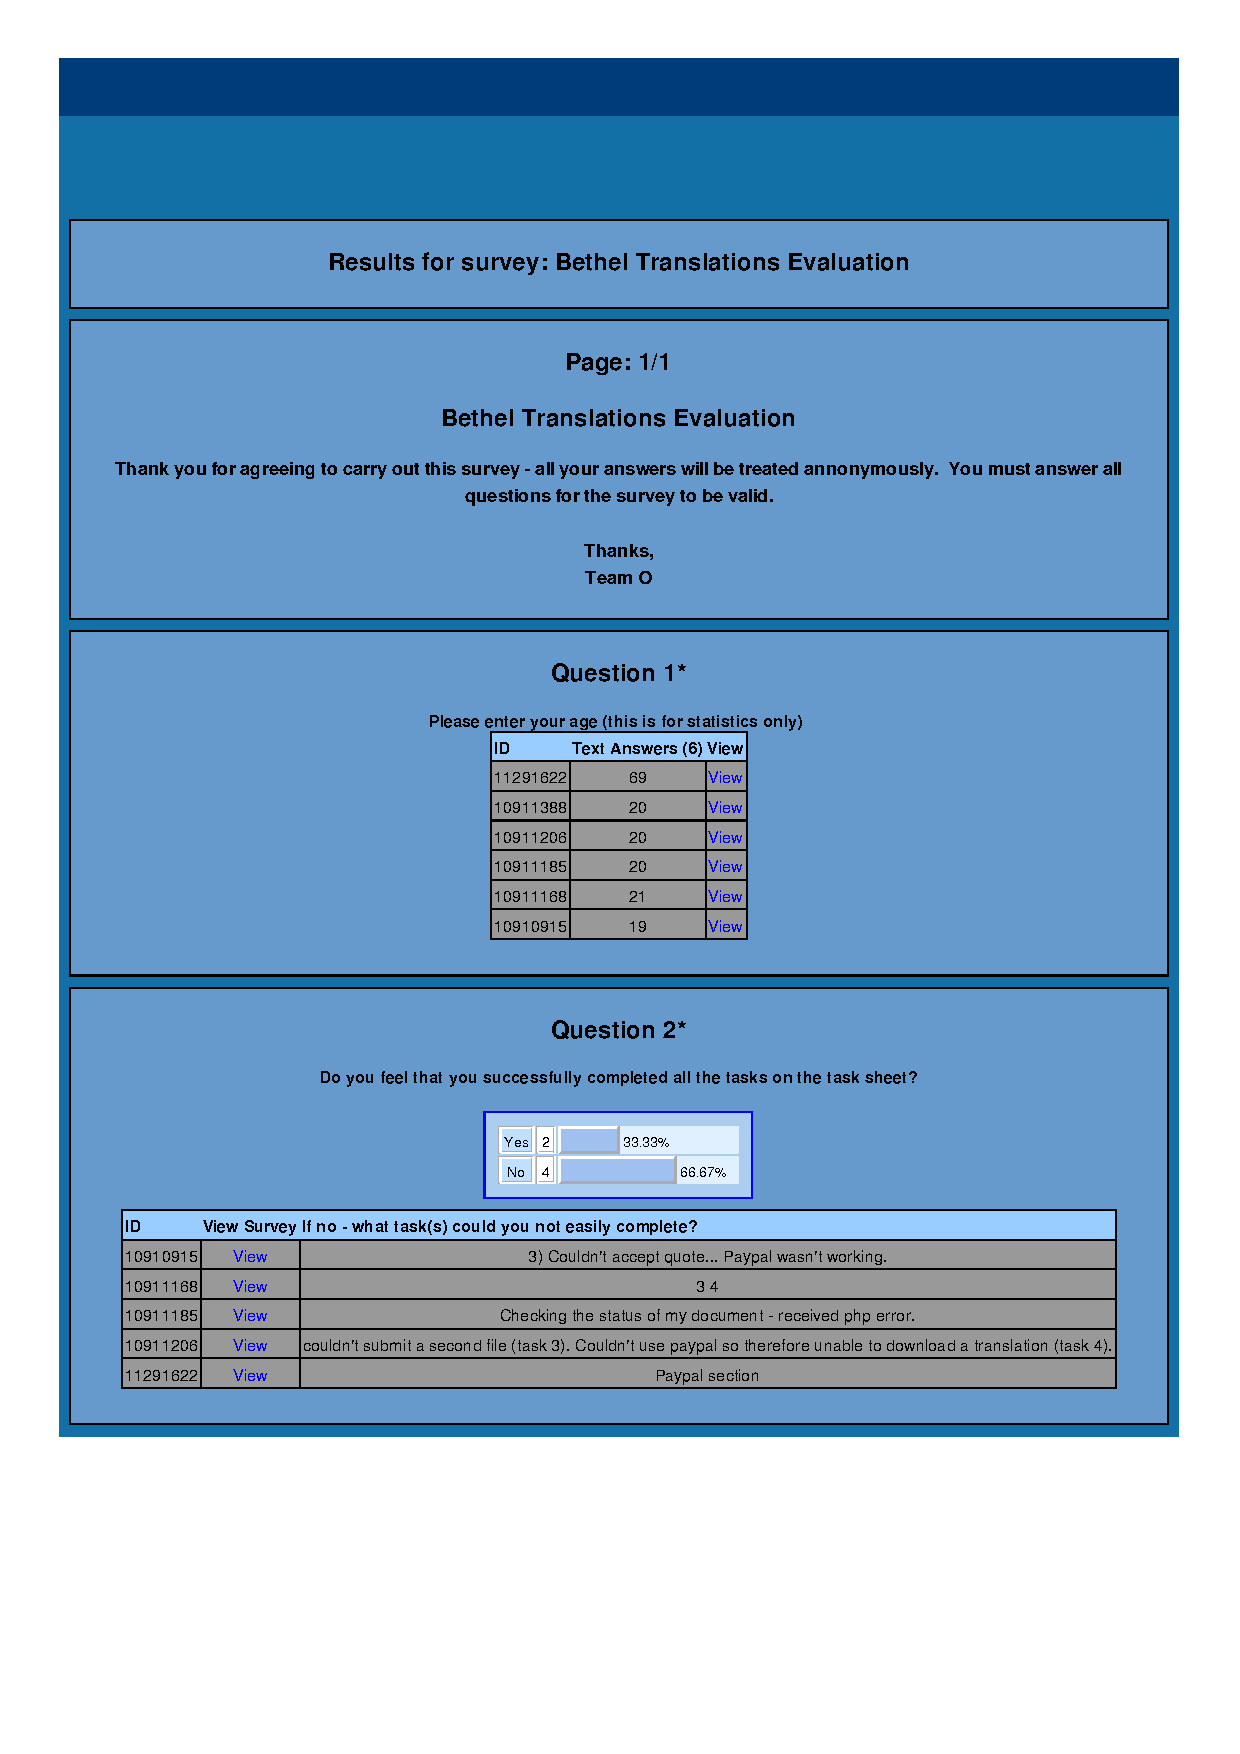
\includepdf[pages={-}]{images/survey-results.pdf}
%-----------------------------------------------------------------------------%
\chapter{Summary Log and Status Report}
The software system is in a completed state. It is currently live on \url{http://www.betheltranslations.com} and is available to be used
by the general public. The only thing that currently needs to be fixed is to change the payment action to a real PayPal business account instead of
the testing sandbox we have set up.

Other than this a potential customer is able to come to the site, find out all the information that they may need to make an educated decision
about whether or not to use Bethel Translations and then to upload their documents for quotation. The translator can then carry out the process
of quoting the user's documents and follow the process through to completion.

From our evaluation we believe that customers will find the system intuitive to use, however we have left Jo\"{e}lle with a user manual to aid
her use of the system, and we are now running a one month beta test. Should she have any problems she will get back in touch with us and if possible
we will try to address any issues that may arise, after our examinations, during the summer break.
 
    


\end{document}
